%%%%%%%%%%%%%%%%%%%%%%%%%%%%%%%%%%%%%%%%%%%%%%%%%%%%%%%%%%%%%%%%%%%%%
%%                                                                 %%
%% Please do not use \input{...} to include other tex files.       %%
%% Submit your LaTeX manuscript as one .tex document.              %%
%%                                                                 %%
%% All additional figures and files should be attached             %%
%% separately and not embedded in the \TeX\ document itself.       %%
%%                                                                 %%
%%%%%%%%%%%%%%%%%%%%%%%%%%%%%%%%%%%%%%%%%%%%%%%%%%%%%%%%%%%%%%%%%%%%%

%%\documentclass[referee,sn-basic]{sn-jnl}% referee option is meant for double line spacing

%%=======================================================%%
%% to print line numbers in the margin use lineno option %%
%%=======================================================%%

%%\documentclass[lineno,sn-basic]{sn-jnl}% Basic Springer Nature Reference Style/Chemistry Reference Style

%%======================================================%%
%% to compile with pdflatex/xelatex use pdflatex option %%
%%======================================================%%

%%\documentclass[pdflatex,sn-basic]{sn-jnl}% Basic Springer Nature Reference Style/Chemistry Reference Style

%%\documentclass[sn-basic]{sn-jnl}% Basic Springer Nature Reference Style/Chemistry Reference Style
\documentclass[sn-mathphys]{sn-jnl}% Math and Physical Sciences Reference Style
%%\documentclass[sn-aps]{sn-jnl}% American Physical Society (APS) Reference Style
%%\documentclass[sn-vancouver]{sn-jnl}% Vancouver Reference Style
%%\documentclass[sn-apa]{sn-jnl}% APA Reference Style
%%\documentclass[sn-chicago]{sn-jnl}% Chicago-based Humanities Reference Style
%%\documentclass[sn-standardnature]{sn-jnl}% Standard Nature Portfolio Reference Style
%%\documentclass[default]{sn-jnl}% Default
%%\documentclass[default,iicol]{sn-jnl}% Default with double column layout

%%%% Standard Packages
%%<additional latex packages if required can be included here>
%%%%

%%%%%=============================================================================%%%%
%%%%  Remarks: This template is provided to aid authors with the preparation
%%%%  of original research articles intended for submission to journals published 
%%%%  by Springer Nature. The guidance has been prepared in partnership with 
%%%%  production teams to conform to Springer Nature technical requirements. 
%%%%  Editorial and presentation requirements differ among journal portfolios and 
%%%%  research disciplines. You may find sections in this template are irrelevant 
%%%%  to your work and are empowered to omit any such section if allowed by the 
%%%%  journal you intend to submit to. The submission guidelines and policies 
%%%%  of the journal take precedence. A detailed User Manual is available in the 
%%%%  template package for technical guidance.
%%%%%=============================================================================%%%%

\jyear{2021}%

%% as per the requirement new theorem styles can be included as shown below
\theoremstyle{thmstyleone}%
\newtheorem{theorem}{Theorem}%  meant for continuous numbers
%%\newtheorem{theorem}{Theorem}[section]% meant for sectionwise numbers
%% optional argument [theorem] produces theorem numbering sequence instead of independent numbers for Proposition
\newtheorem{proposition}[theorem]{Proposition}% 
%%\newtheorem{proposition}{Proposition}% to get separate numbers for theorem and proposition etc.

\theoremstyle{thmstyletwo}%
\newtheorem{example}{Example}%
\newtheorem{remark}{Remark}%

\theoremstyle{thmstylethree}%
\newtheorem{definition}{Definition}%
\usepackage{tabularray}
\definecolor{MineShaft}{rgb}{0.2,0.2,0.2}

\usepackage{subfigure}
\usepackage{multirow}
\usepackage{color}
\usepackage{float}
\usepackage{amsmath,epsfig}
\usepackage{amssymb}
\usepackage[justification=centering]{caption}

\raggedbottom
%%\unnumbered% uncomment this for unnumbered level heads

\begin{document}

\title[Article Title]{Texture-aware Re-parameterization to Mitigate Accuracy Drop after Quantization for 4K/8K Image Super-resolution}

\author[1]{\fnm{Yongxu} \sur{Liu}}\email{2211002057@cnu.edu.cn}

\author*{\fnm{Xiaoyan} \sur{Fu}\textsuperscript{2,*}}\email{fuxiaotriumph@163.com}

\author{\fnm{Zhong} \sur{Sun}\textsuperscript{3}}\email{5689@cnu.edu.cn}

\affil[1,2,3]{\orgdiv{College of Information Engineering}, \orgname{Capital Normal University}, \orgaddress{ \street{Haidian District}, \city{Beijing}, \postcode{100089}, \country{China}}}


\abstract{In this paper, we aim to improve super-resolution (SR) imaging quality on 4K/8K images with a negligible increase in computational cost and alleviate the accuracy drop after quantization. Experiments have discovered two phenomena: (i) the re-parameterization (Rep) technique has no apparent advantages in regions with smooth textures, and (ii) the accuracy drop after quantization compared with SR methods based on No-Rep because the structure information of the image will be weakened caused by the multi-branch fusion in Rep technique. Inspired by the above phenomenon, we innovatively combine texture classification and Rep techniques to propose a generic TARepSR framework (consisting of TA-Module and VarRepSR-Module) to adjust the branching of Rep blocks texture-awarely. Specifically, the TA-Module is a lightweight classification network to classify textures in different regions. An existing SR network using texture-aware Rep techniques can be used as the VarRepSR-Module to super-resolute images with higher imaging quality without additional computational costs. Moreover, we propose a TC loss to avoid over-fitting caused by an unbalanced degree of the tendency of classification results to classify different textures better. Experiments show that our TARepSR can not only improve the imaging quality of most existing methods (e.g., FSRCNN, CARN, EDSR, XLSR) on 4K/8K images with negligible increase in computational cost but also improve the accuracy after quantization compared with the state-of-the-art Rep methods.}

\keywords{super-resolution, re-parameterization, model quantization}

%%\pacs[JEL Classification]{D8, H51}

%%\pacs[MSC Classification]{35A01, 65L10, 65L12, 65L20, 65L70}

\maketitle

\section{Introduction}\label{sec1}
Image super-resolution (SR) aims to generate corresponding high-resolution (HR) images from degraded low-resolution (LR) images. In recent years, the display resolution of many smartphones and TV monitors have reached HR levels, such as 4K (4096$\times$2160) and 8K (7680$\times$4320). However, the current mainstream image/video sources are still dominated by 720P and 1080P, which limits the quality of the image/video system from the source end \cite{EGVSR,mobile2,mobile3,ARM}. Therefore, there is an urgent need for a deployment-friendly and quantization-friendly SR model in real life to reconstruct LR images to 4K/8K images with higher imaging quality to solve the shortage of HR image/video sources.

In general, complex SR models are difficult to be deployed directly on hardware devices with limited resources because of their expensive computational costs \cite{mobile1,RealBasicVSR,basicvsr++,CBAM,DRRN,RCAN,liu2022cross,yang2021image,MFFN}. Recently, researchers have used structural re-parameterization techniques (Rep) \cite{RepVGG,ACnet,DBB}, and their variants \cite{Dyrep,RepBN,ECB,EDBB,OREPA} to reconstruct SR images with sharper textures without adding additional computational cost, which has emerged as a leading strategy to solve the above problem. The biggest highlight of the structurally-reparameterized SR method is that the structure of the model used for the training and inference phases is different. Typical examples include ECB \cite{ECB} and EDBB \cite{EDBB}, which extend convolution with multiple branches during the training phase. Then, these branches are fused into an original convolution in the inference phase to achieve inference with low computational cost without an accuracy drop. Moreover, the same structurally-reparameterized block is often accepted to reconstruct all pixels of an image in recent work \cite{RepVGG,ACnet,DBB,ECB,EDBB,OREPA}, and we call this strategy as ``Global-Rep".

Numerical experiments have discovered two phenomena: (i) Rep technique has no apparent advantages in regions with smooth textures (smooth regions usually account for more than 50\%, see Figure~\ref{texture_distribution}), and (ii) the accuracy drop after quantization compared with SR methods based on No-Rep (see Table~\ref{tab:quan1}). Phenomenon (i) indicates that the ``Global-Rep" method is used for different textures and might not be the best solution. The reason for the phenomenon (ii) is that the structural information of the image may be weakened during the merging of multiple branches, which means that it is necessary to reduce unnecessary multi-branch fusion in regions with smooth textures. Thus, the above premise motivates us to adaptively adjust the structure of the re-parameterized blocks and the network structure according to the texture of the LR images.

\begin{figure}
    \centering
    % \setlength{\abovecaptionskip}{0.cm}
    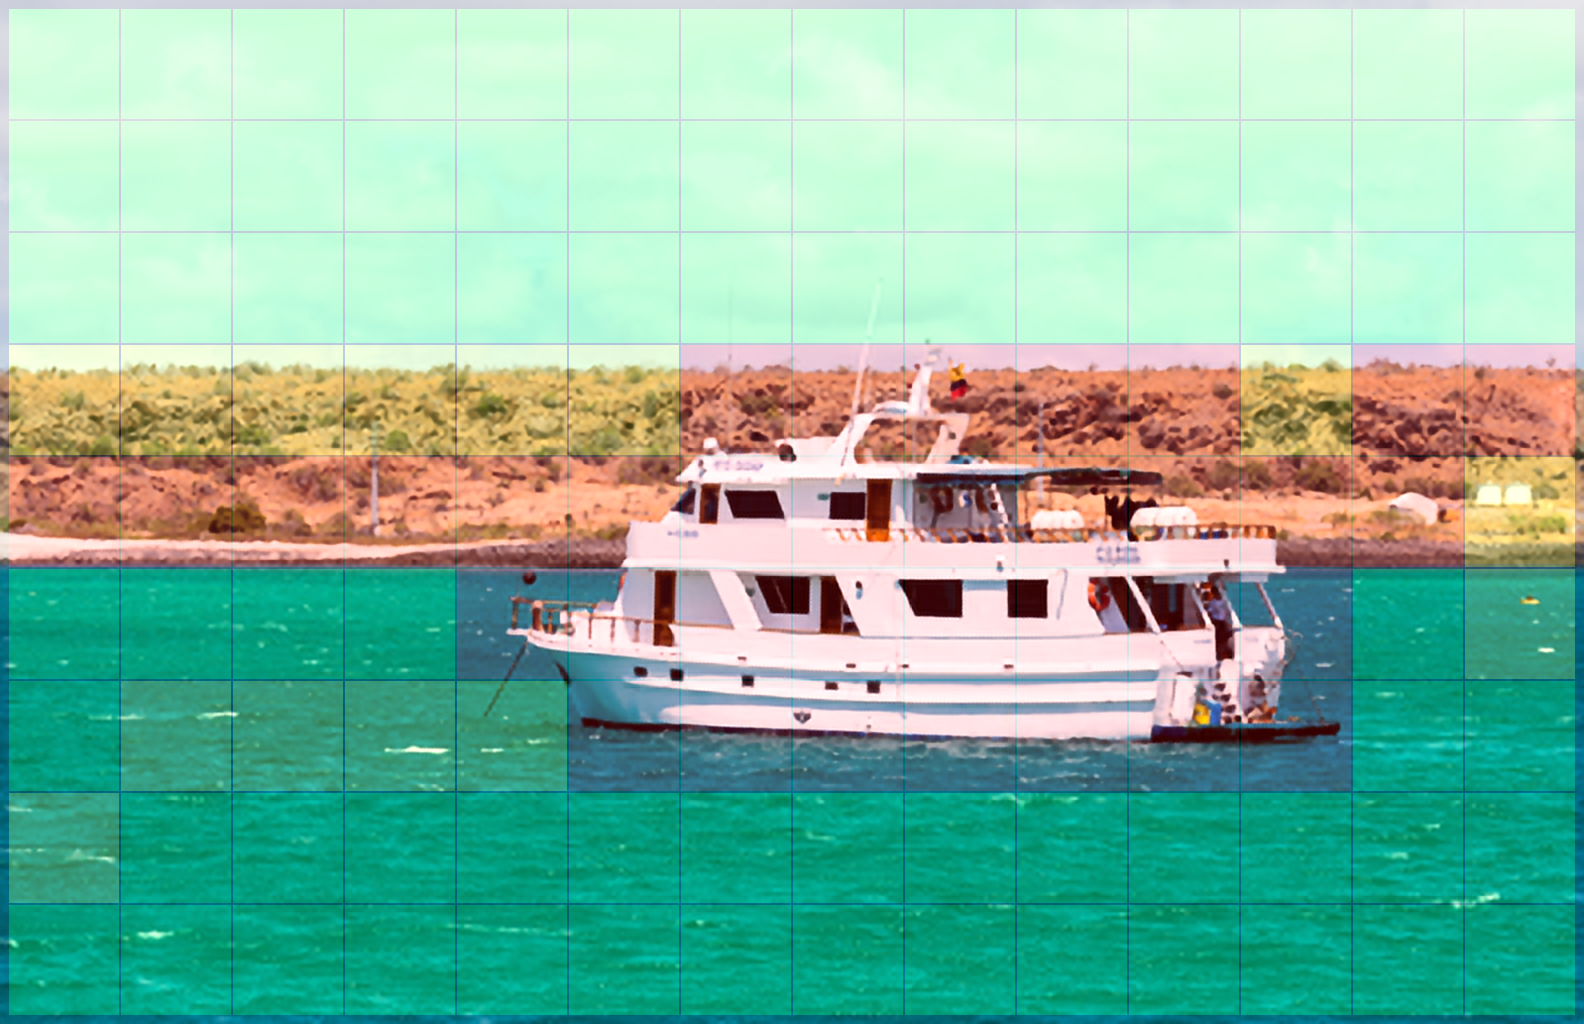
\includegraphics[width=2.5in]{1217_mask.png}
    \caption{``1217" (DIV8K) into 66\% smooth (green), 6\% medium (yellow), and 28\% complex (red) textures.}
    \label{texture_distribution}
\end{figure}

In this paper, we propose a general TARepSR framework (consisting of the TA and VarRepSR modules), which can be considered the texture-aware ``Local-Rep'' strategy rather than ``Global-Rep''. It can achieve two improvements: (i) the imaging quality is improved with a negligible increase in computational cost, and (ii) adaptive simplification of branching in regions with smooth textures to mitigate the accuracy drop due to multi-branch fusion after quantization. Specifically, we propose a re-parameterized block with a variable structure (VarRep) consisting of a branch selector and different branches. TA-Module is a lightweight classification network to classify various regions into three categories (``Smooth", ``Medium," and ``Complex") based on texture complexity. An existing SR network using VarRep can be used as the VarRepSR-Module to super-resolute various image regions with higher imaging quality. Regarding the loss function, the $\ell_1$ loss is used to guarantee the essential performance. Further, we observe that the overwhelming majority of regions are easily classified to the most complex textures because the most complex VarRep easily gives better results. We hope the classification results are more inclined to ``Smooth". Therefore, we propose a texture classification loss function (TC loss) to classify different textures better. To validate the effectiveness of the proposed TARepSR framework, we apply it to some existing SR networks. Experimental results show that the proposed TARepSR framework can improve the imaging quality of these SR networks by $\sim$0.1dB on 4K/8K images with negligible increase in computational cost. In addition, the accuracy drop of our strategy after quantization is reduced by $\sim$0.15dB on average compared to the state-of-the-art (SOTA) SR methods based on Global-Rep, which facilitates the practical deployment of the model on mobile devices.

\begin{figure*}[htbp]
    \centering
    % \setlength{\abovecaptionskip}{0.cm}
    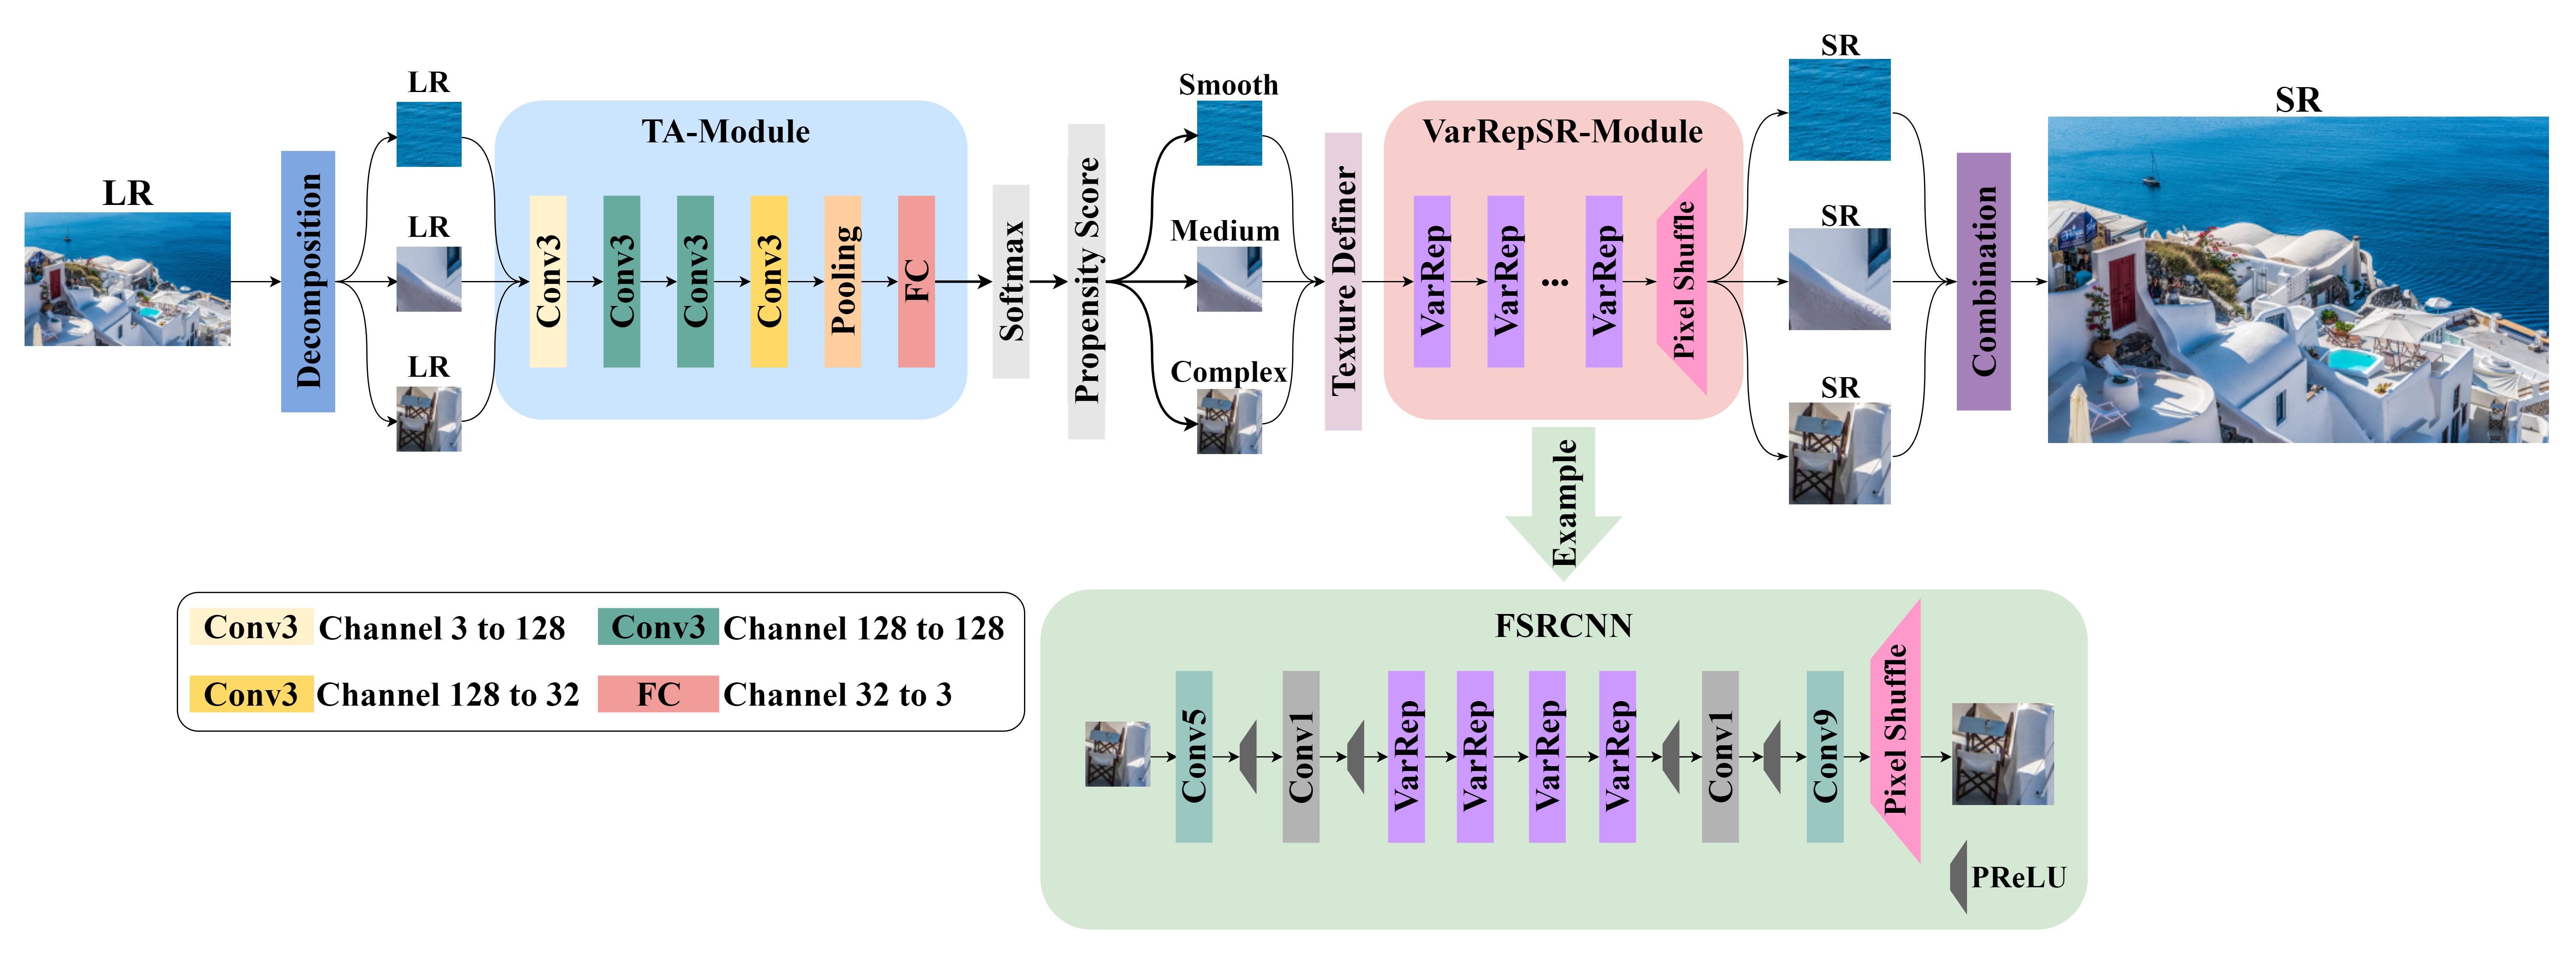
\includegraphics[width=4.9in]{main-4.png}
    \caption{The overview of the proposed TARepSR framework.}
    \label{TARepSR}
\end{figure*}

Our main contributions can be summarized as follows.

(1) We explore the effectiveness of Rep techniques in regions with different textures and propose a texture-aware ``Local-Rep'' strategy rather than ``Global-Rep''. It aims to reduce using complex branches in regions with smooth textures, thus alleviating the accuracy drop after quantization caused by multi-branch fusion.

(2) Based on the ``Local-Rep" strategy, we propose a general TARepSR framework, which can be applied with existing SR networks to improve their imaging quality on 4K/8K images with negligible increase in computational cost.

(3) In training, we classify different regions of an image according to how hard they are recovered rather than traditional classification methods and propose a TC loss to avoid over-fitting caused by an unbalanced degree of the tendency of classification results to classify different textures better.

\section{Related Works}
\subsection{Re-parameterization}
The re-parameterization technique is widely accepted in the field of SR because of its ability to effectively improve the SR performance without adding additional computational cost, such as RepVGG \cite{RepVGG}, ACNet \cite{ACnet}, ECB \cite{ECB}, and EDBB \cite{EDBB}. In general, complex re-parameterized blocks in the above methods are designed to process all the pixels of an image. However, the effectiveness of the re-parameterization in regions with different textures raises our concern, which will be discussed in Section 2.2.

\subsection{Analysis of re-parameterization before/after quantization}
\begin{table}[htbp]
    \centering
    \caption{PSNRs of re-parameterizable blocks in different texture regions. Text: Before/After quantification.}
    \resizebox{11cm}{!}{
    \begin{tabular}{cccc} 
    \toprule
    Model  & Smooth            & Medium            & Complex            \\ 
    \midrule
    No-Rep & 42.70dB~/ 39.86dB & 29.69dB~/ 25.63dB & 22.73dB / 17.47dB  \\
    ECB \cite{ECB}    & 42.72dB~/ 39.76dB & 29.76dB~/ 25.62dB & 22.91dB / 17.52dB  \\
    EDBB \cite{EDBB}   & 42.72dB~/ 39.73dB & 29.78dB~/ 25.62dB & 22.98dB / 17.54dB  \\
    \bottomrule
    \end{tabular}
    }
    \label{tab:quan1}
\end{table}

\begin{figure}[H]
    \begin{center}
    % \setlength{\abovecaptionskip}{0.cm}
    
\includegraphics[width=4in]{texture.png}
    \caption{Images from DIV2K with different textures.}
    \label{texture}
    \end{center}
\end{figure} 

Wang $et\,al.$ \cite{SMSR} proposed a method and criteria for classifying textures based on texture complexity by learning sparse masks. Inspired by Wang, we used their method and criteria to classify the various regions of the images in the DIV2K \cite{Div2K} dataset as ``smooth'', ``medium'' and ``complex'' based on texture complexity (see Figure~\ref{texture}). Based on this processing, we observe that the texture distribution of an image is uneven (see Figure~\ref{texture_distribution}), where regions with complex textures only account for 20$\sim$30\%. In contrast, smooth regions account for more than 50\%. This phenomenon is more evident in large images such as 4K/8K. To analyze the effectiveness of the re-parameterizable block for different texture regions (see Table~\ref{tab:quan1}), we test different re-parameterizable blocks (e.g., ECB \cite{ECB}, EDBB \cite{EDBB}, and No-Rep.) in three regions with smooth, medium and complex textures, respectively. Two phenomena have been discovered by the above experiments as follows.

(i) The advantage of the re-parameterization technique decreases as the smoothness of the texture increases.

(ii) The accuracy drop after quantization compared with SR methods without re-parameterization technique (No-Rep). 

\begin{table}
\centering
\caption{The accuracy drop after quantization with different numbers of multi-branch fusions.}
\resizebox{7cm}{!}{
\begin{tabular}{cccc} 
\toprule
Model     & Before(dB) & After(dB) & Drop(dB)  \\ 
\midrule
Branch(1) & 25.61      & 19.72     & 5.89      \\
Branch(2) & 25.63      & 19.71     & 5.92      \\
Branch(3) & 25.67      & 19.71     & 5.96      \\
Branch(4) & 25.69      & 19.65     & 6.04      \\
\bottomrule
\end{tabular}
}
\label{tab:multi-branch}
\end{table}

Phenomenon (i) indicates that the ``Global-Rep" method is simply used for different textures and might not be the best solution, which motivates us to design different re-parameterization techniques in regions with different textures. In addition, when deploying deep learning models to mobile devices, it is widespread to use quantization processing, especially unit8 quantization, which is supported by many mobile devices. Ding $et\,al.$ \cite{RepOpt} reveal that the structural conversion (i.e., BN fusion and multi-branch fusion in re-parameterization) cause the quantization-unfriendly parameter distribution. Inspired by Ding, we analyze the reasons for the phenomenon (ii) by an experiment. Our experiments test the accuracy drop after quantization with different numbers of multi-branch fusions (see Table~\ref{tab:multi-branch}). Specifically, we use multi-duplicate 3$\times$3 convolution block as the re-parameterized block, and Branch($n$) denotes the re-parameterized block with $n$ branches, i.e., Figure~\ref{re-perameterization_blocks}(a) represents Branch($3$). As can be seen in Table~\ref{tab:multi-branch}, the accuracy drop after quantization gradually with the increase of the number of branches, which means that the structural information of the image may be weakened during the merging of multiple branches and thus lead to accuracy drop after quantization. Therefore, phenomena (i) and (ii) can provide us with a motivation that it is necessary to reduce unnecessary multi-branch fusion in regions with smooth textures.

\begin{figure}[h!]
    \centering
    % \setlength{\abovecaptionskip}{0.cm}
    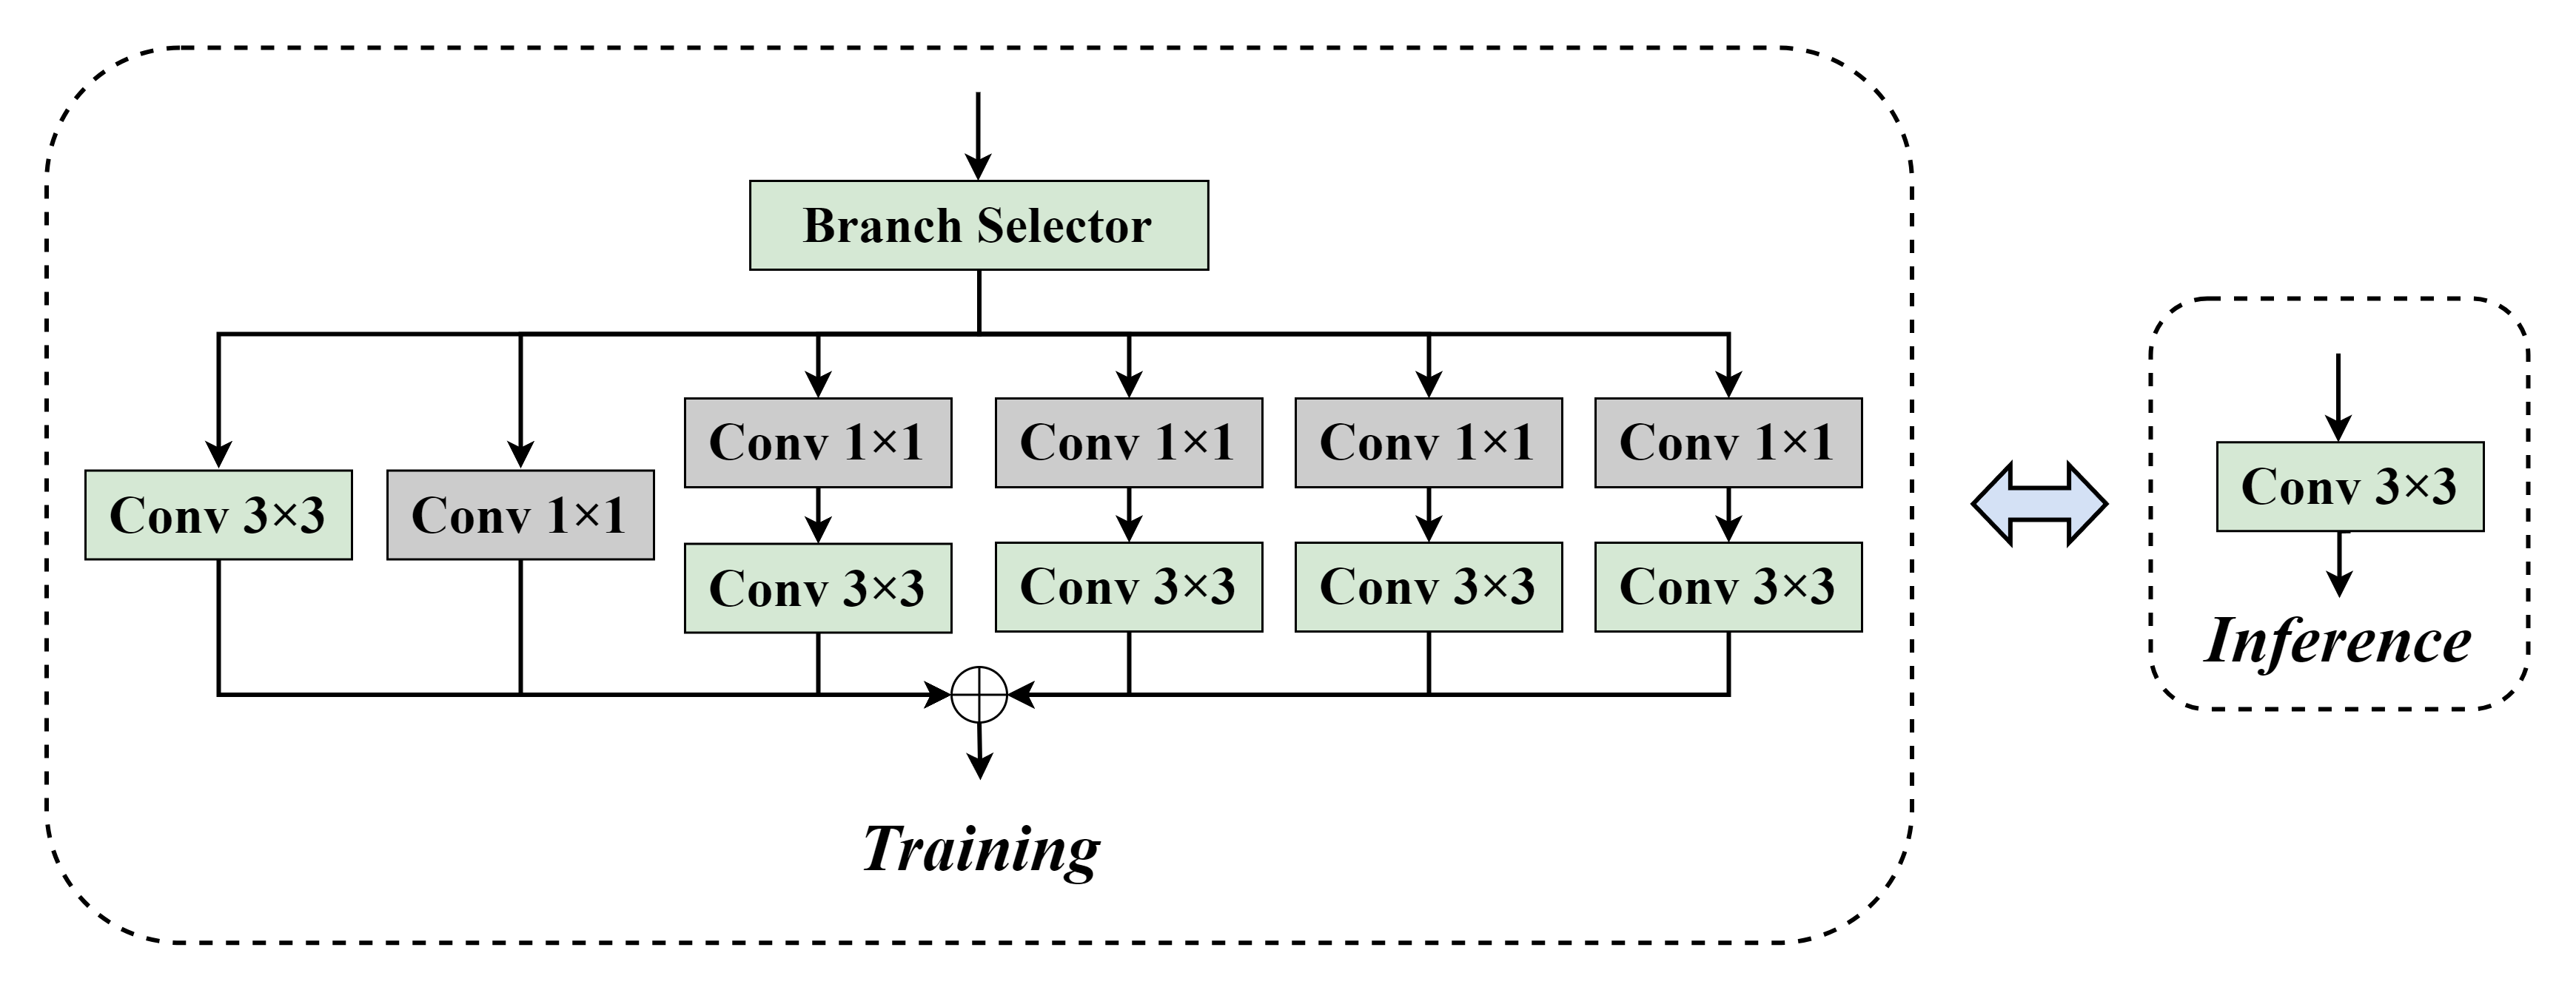
\includegraphics[width=3.6in]{VarRep2.png}
    \caption{Re-parameterized block with variable structure.}
    \label{VarRep}
\end{figure} 

\section{Proposed Method}
\subsection{VarRep block}
This paper proposes a re-parameterized block with a variable structure (VarRep) to reduce excessive branches used in unnecessary cases (e.g., in regions with smooth textures). VarRep consists of branch selectors and different branches, and its structure is shown in Figure~\ref{VarRep}. In the branch selector, the indexes of the different branches are stored in an array $S[0,0, \ldots, 0]$, where the current branch is one if it is selected and 0 if it is not, e.g., $[1,0,1,0,0,0]$ means that only the first and third branches are selected. Then, VarRep reconstructs a new re-parameterized block based on the branch selection. The different branches are defined as follows.

\textbf{Branch I and II: A vanilla 1$\times$1 and 3$\times$3 convolution.} We first use an ordinary 1$\times$1 and 3$\times$3 convolution as the first and second branches of VarRep to ensure the basic performance. Unlike the re-parameterized blocks in high-level computer vision tasks, the BN layer \cite{BN} is not used because it hinders the merging of different branches and costs significant computational overhead. The ordinary 1$\times$1 and 3$\times$3 convolutions are represented as follows.

\begin{equation}
\begin{aligned}
&f_1(X)=W_1 * X+n_1 \\
&f_2(X)=W_2 * X+n_2
\end{aligned}
\end{equation}

Where $X$, $\left\{W_1, W_2\right\}$ and $\left\{n_1, n_2\right\}$ denote the input features, weights, and biases, respectively.

\textbf{Branch III-VI: Sequential convolution.} Sequential convolution can further extract the hidden information from the feature mapping efficiently. In VarRep, we introduce sequential convolution to enhance the texture and structure signals of SR images, which are represented as follows.

\begin{equation}
f_S(X)=W_{S_2} *\left(W_{S_1} * X+n_{S_1}\right)+n_{S_2}
\end{equation}

Where $X$ denotes the input features, $\left\{W_1, n_1\right\}$ denotes the weights and biases of the first convolution with $D \times C \times 1 \times 1$, $\left\{W_2, n_2\right\}$ denotes the weights and biases of the second convolution with $D \times C \times 3 \times 3$, $*$ denotes the regular convolution operation. To merge them into a $C \times C \times K \times K$ convolution with $\left\{W_s, b_s\right\}$, we can obtain the transformation based on \cite{DBB} as follows.

\begin{equation}
\begin{aligned}
&W_S=\operatorname{perm}\left(W_1\right) * W_2 \\
&n_S=W_2 * \operatorname{rep}\left(n_1\right)+n_2
\end{aligned}
\end{equation}

Where $\operatorname{perm}()$ denotes the operation of exchanging the one and two dimensions of the tensor, and $\operatorname{rep}()$ denotes the spatial broadcasting operation, e.g., $n \in \mathbb{R}^{C \times 1 \times 1 \times 1}$ and $\operatorname{rep}(n) \in \mathbb{R}^{C \times 1 \times 3 \times 3}$.

Then, we describe how to re-parameterize the VarRep block into a regular 3$\times$3 convolution for efficient inference. Suppose the first three branches of VarRep are selected (the same operation can be used on the third through sixth branches since they are the same). We use $\left\{W_{rep}, n_{rep}\right\}$ to denote the weights and biases of a regular 3$\times$3 convolution that is used for inference. The final weights and biases after re-parameterization are as follows.

\begin{equation}
\begin{aligned}
&W_{r e p}=W_1+W_2+W_S \\
&n_{r e p}=n_1+n_2+n_S \\
&F(X)=W_{r e p} * X+n_{r e p}
\end{aligned}
\end{equation}

\subsection{Overview of TARepSR framework}
In this section, we describe the architecture and steps of the proposed TARepSR, which consists of the TA-Module and the VarRepSR-Module, as shown in Figure~\ref{TARepSR}. To emphasize, the design idea of the TARepSR framework is the proposed texture-aware ``Local-Rep'' strategy, i.e., the Rep technique can be adaptively adjusted according to the texture. Specifically, a complete LR image is decomposed into $N$ sub-images, denoted as $\left\{x_1, x_2, \ldots, x_N\right\}$. The TA-Module (see Section 2.4) serves to group sub-images into three categories (``Smooth", ``Medium," and ``Complex") according to the complexity of the texture. Then, the classified sub-images are super-resolved by VarRepSR-Module (see Section 2.5) respectively, and the super-resolved sub-images are recorded as $X_i=F_{S R}\left(x_i\right)$. Finally, all reconstructed sub-images $X_i$ are stitched into a large SR image $X$ (4K/8K).

\subsection{TA-Module}
The role of the TA-Module is to determine whether the texture of the sub-image is smooth, medium, or complex. It consists of four convolution layers, an average pooling layer, and a fully-connected layer (see Figure~\ref{TARepSR}). The computational cost of the TA-Module is negligible, and it does not contain components and structures that are not friendly to quantification. In training, TA-Module classifies sub-images according to how easily they are recovered rather than classifying images according to predefined labels as in traditional classification networks.

Next, we describe the specific classification methods in training and testing.

In training, the sub-image $x_i$ is super-resolved by VarRep with simple, medium, or complex branches, and the super-resolved result is defined as $F_{S R}^j\left(x_i\right)$ ($x \in \left\{1,2, \ldots, N\right\}$, $j \in \left\{1,2,3\right\}$). Then, the output data after the FC layer is normalized using the $Softmax(\cdot)$, and the normalized data is defined as the propensity score of classification $\left\{\eta_i^1, \eta_i^2, \eta_i^3\right\}$. Finally, the super-resolved sub-image $F_{S R}^j\left(x_i\right)$ is multiplied by the corresponding propensity score $\left\{\eta_i^1, \eta_i^2, \eta_i^3\right\}$ to ensure that the TA-Module can accept the gradient propagation from the reconstruction results. The final SR output $x_i$ is as follows.

\begin{equation}
x_i=\sum_{j=1}^3 \eta_i^j \times F_{S R}^j\left(x_i\right)
\end{equation}

In testing, we choose the classification with the largest propensity score $\left\{\eta_i^1, \eta_i^2, \eta_i^3\right\}$ ($x \in \left\{1,2, \ldots, N\right\}$) as the texture classification of the current sub-image $x_i$.

\begin{figure}
    \centering
    \subfigure[Multi-duplicate block]{\includegraphics[width=3.4cm]{Triple_3×3.png}} 
    \raisebox{-0.01\height}{
        \subfigure[ECB \cite{ECB}]{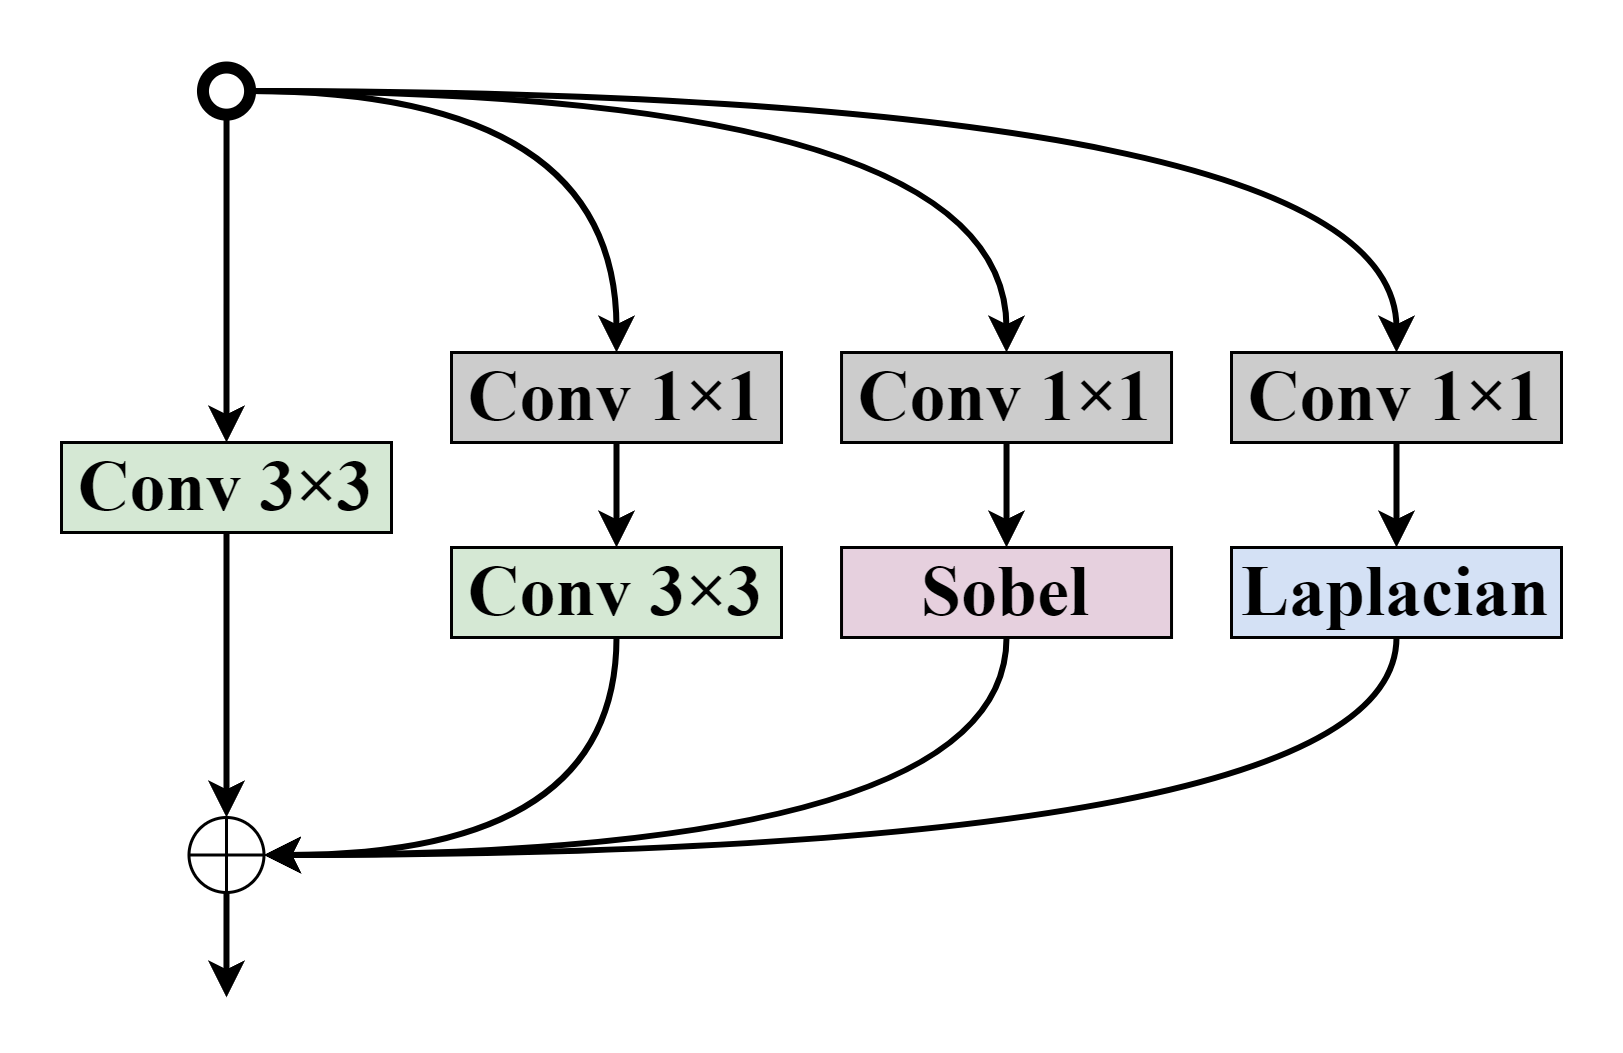
\includegraphics[width=4cm]{ECB2.png}}
    }
    \\
    \centering
    \subfigure[EDBB \cite{EDBB}]{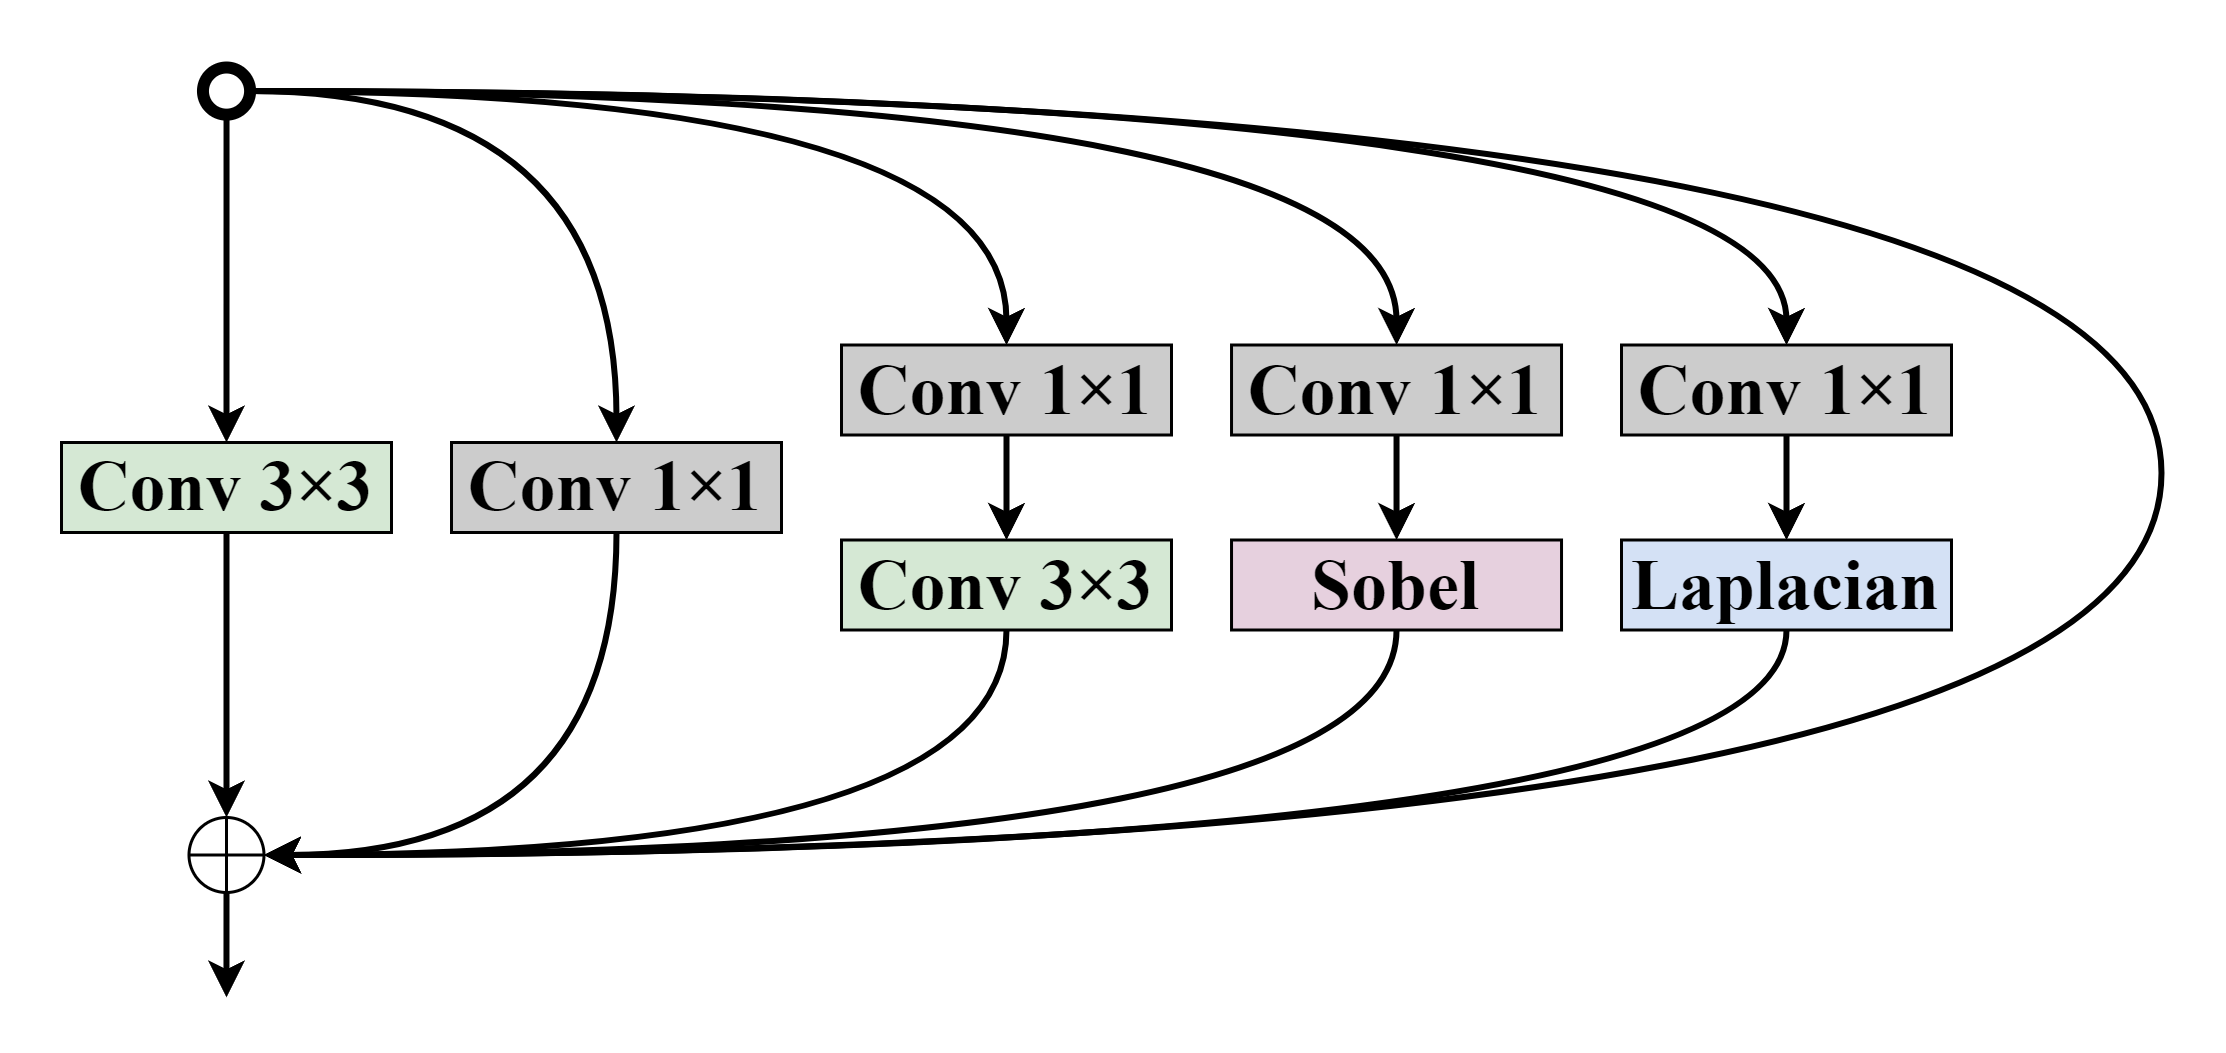
\includegraphics[width=5cm]{EDBB2.png}}
    \vspace{-0.2cm}
    \caption{Architectures of the compared re-parameterization blocks.}
    \label{re-perameterization_blocks}
\end{figure}

\subsection{VarRepSR-Module}
There is a texture definer before VarRepSR-Module, which defines the array $S$ of the texture selector of VarRep according to the texture classification. In this paper, we define $S[1,1,0,0,0,0]$ (VarRep-S) for smooth textures, $S[1,1,1,1,0,0]$ (VarRep-M) for medium textures and $S[1,1,1,1,1,1]$ (VarRep-L) for complex textures. The VarRepSR-Module can be seen as an SR network container, an existing SR network. Note that the 3$\times$3 convolution in the depth feature extraction layer of the existing network needs to be replaced with our VarRep block.

\subsection{Loss function}
This paper's loss function includes the regular $\ell_1$ loss and the proposed TC loss. Specifically, $\ell_1$ loss ensures the essential SR quality ($\ell_1=\frac{\sum_{i=1}^N \rvert f\left(x_i\right)-y_i \rvert}{N}$, where $f\left(x\right)$ denotes the predicted value, $y$ denotes the true value and $N$ denotes the number of samples.). In addition, we observe that the sub-images are easily classified as the most complex textures because the most complex VarRep easily gives better results. We hope the classification results are inclined to ``Smooth'' and ``Medium'' since these regions account for more than 70\% of the whole image. Therefore, we propose a texture classification loss function (TC loss) to classify better the different textures, which is formulated as

\begin{equation}
\ell_{T C}=\rvert \sum_{i=1}^N \eta_1\left(x_i\right)-\alpha N \rvert+\rvert \sum_{j=1}^N \eta_2\left(x_j\right)-\beta N \rvert
\end{equation} 

Where $N$ denotes the number of sub-images, $\alpha$ and $\beta$ ($0<\alpha+\beta<1$) denote the degree of tendency toward smooth and medium textures, respectively ($\alpha$ and $\beta$ are set to 0.5 and 0.2 in this paper).
$\sum_{i=1}^N \eta_1\left(x_i\right)$ and $\sum_{j=1}^N \eta_2\left(j_i\right)$ denote the number of sub-images classified as texture smooth and medium, respectively. Finally, the definition of our loss function is shown as follows.

\begin{equation}
\ell=\lambda_1 \times \ell_1+\lambda_2 \times \ell_{T C}
\end{equation}

Where $\lambda_1$ and $\lambda_2$ are the weights to balance the different loss terms and $\ell_1$ denotes the 1-norm distance between the output image and the actual image.

\subsection{Other details of TARepSR}
\textbf{Regarding to BN layer.} Unlike the re-parameterized blocks in high-level computer vision tasks, the BN layer \citep{BN} is not accepted. In SR, the output image must be identical to the input in terms of color, contrast, and brightness, and only the resolution and some texture details need to be changed. However, the BN layer stretches the image's contrast, and the color distribution is normalized. In other words, the BN layer destroys the original contrast information of the image, which means that it affects the imaging quality and the stability of the training.

\textbf{Complexity of VarRep block.} In this paper, we aim to propose a new idea and framework based on classification discussion, i.e., the different re-parameterization techniques in regions with different textures are used. Therefore, the design of VarRep is more straightforward than DBB \citep{DBB} or EDBB \citep{EDBB}, and our method proves that the SR performance is improved with a relatively simple design. Note, although the branch design is not fixed, we believe that a $3\times3$ convolution and a $1\times1$ convolution used in regions with simple texture is sufficient, and model quantization will be compromised by overly complex multi-branch fusion.


\section{Experiments}
\subsection{Settings}
\textbf{Datasets and metrics.} The widely used Div2K \cite{Div2K} is used as the training dataset. We did not use the commonly used SR test sets, e.g., Set5 \cite{set5}, Set14 \cite{set14}, and Urban100 \cite{urban100} because their images are too small for sub-image decomposition. We selected 200 images from the DIV8K \cite{div8k} dataset and downsampled them (the downsampling method is Bicubic) to 2K (100 images) and 4K (100 images) resolutions to serve as HR images for the Test2K and Test4K test sets. The evaluation metrics are the peak signal-to-noise ratio (PSNR) and floating-point operations per second (FLOPs). 

\textbf{Training details.} We divide 800 training images into two groups in the training, where the first 790 images are used for training, and the last ten images are used for validation. For the training strategy, we train TA-Module and VarRepSR-Module separately. Specifically, we first train the SR networks of VarRep with three different complexities separately, i.e., train the VarRepSR-Module. Then, the TA-Module is iteratively trained 200k times using the proposed loss function because the performance is volatile and challenging to converge if the TA-Module and VarRepSR-Module are trained simultaneously. Finally, we train the two modules jointly, keeping all settings constant.

\textbf{Implementation details.} Before training, LR images of size $32\times32$ are randomly cropped, and the intensity of the images is randomly adjusted to 1, 0.7, or 0.5 to be more robust to illumination changes. The mini-batch size is set to 16, and Adam \cite{adam} ($\beta_1=0.9, \beta_2=0.999$) is used as the optimizer. We use the cosine annealing learning strategy to adjust the learning rate, where the initial learning rate is set to $10^{-3}$, the minimum value is set to $10^{-7}$, and the period of cosine is 500k iterations. We set the weights of the loss function to $\lambda_1=2000$ and $\lambda_2=5$. All models are trained and tested on the PyTorch \cite{pytorch} framework and using NVIDIA 2080Ti GPU.


\begin{table*}[h!]
\centering
\label{tab:TARepSR1}
\caption{PSNRs and FLOPs of existing SR networks with TARepSR. 
Red text: best PSNR.}
\resizebox{12cm}{!}{
% \resizebox{\linewidth}{!}{
\begin{tabular}{cc|cc|cc|cc} 
\hline
\multirow{2}{*}{Model } & \multirow{2}{*}{Parameters} & \multicolumn{2}{c|}{Test2K}                             & \multicolumn{2}{c|}{Test4K}                                             & \multicolumn{2}{c}{Test8K}                                                                   \\
                        &                        & PSNR(dB)               & FLOPs(M)                           & PSNR(dB)               & FLOPs(M)                                       & PSNR(dB)               & FLOPs(M)                                                            \\ 
\hline
FSRCNN                  & 25K                    & 25.61                  & 468M~                   & 26.90 & 468M                                    & 32.66                  & 468M                                                          \\
\textbf{FSRCNN-TARepSR} & \textbf{117K}                   & \textcolor{red}{\textbf{25.72}} &\textbf{480M}   & \textcolor{red}{\textbf{27.02}}                  & \textbf{480M} & \textcolor{red}{\textbf{32.76}} & \textbf{480M}                                        \\ 
\hline
CARN                    & 295K                   & 25.95                  & 1.15G                   & 27.34                  & 1.15G                                   & 33.18 & 1.15G                                                        \\
\textbf{CARN-TARepSR}   & \textbf{664K}                   & \textcolor{red}{\textbf{26.06}} & \textbf{1.18G}   & \textcolor{red}{\textbf{27.44}} & \textbf{1.18G}                   & \textcolor{red}{\textbf{33.27}}                  & \textbf{1.18G}                                        \\ 
\hline
EDSR                    & 1.78M                  & 26.08 & 102.85G                 & 27.48 & 102.85G                                 & 33.35 & 102.85G                                                      \\
\textbf{EDSR-TARepSR}   & \textbf{3.94M}         & \textcolor{red}{\textbf{26.17}}     & \textbf{103.02G}  & \textcolor{red}{\textbf{27.56}}                  & \textbf{103.02G}      & \textcolor{red}{\textbf{33.43}}        & \textbf{103.02G}  \\ 
\hline
XLSR                    & 22K                    & 25.77                  & 472M~                   & 27.16                  & 472M                                    & 32.46                  & 472M                                                         \\
\textbf{XLSR-TARepSR}   & \textbf{81K}                    & \textcolor{red}{\textbf{25.88}} & \textbf{486M}   & \textcolor{red}{\textbf{27.28}} & \textbf{486M}                   & \textcolor{red}{32.57} & \textbf{486M}                      \\
\hline
\end{tabular}
}
\end{table*}

\subsection{Re-parameterization after quantification}
In this section, we applied the proposed TARepSR framework to some existing networks (e.g., FSRCNN \cite{FSRCNN}, CARN \cite{CARN}, EDSR \cite{EDSR}, XLSR \cite{XLSR}) to demonstrate that the texture-aware ``Local-Rep" strategy is more friendly to quantification, and compared them with the method based on ``Global-Rep" (e.g., ECB \cite{ECB} and EDBB \cite{EDBB}) on Test2K, Test4K, and Test8K for upscaling factor $\times$4. As seen in Table~\ref{tab:quan2}, the existing network using TARepSR has the highest image quality after quantization and the most negligible accuracy drop compared to No-Rep, ECB, and EDBB, where $\sim$0.11 dB over ECB and $\sim$0.1 dB over EDBB. This experiment demonstrates that our strategy and framework are more friendly to quantification and easier to deploy on mobile devices.

\begin{table*}[h!]
\centering
\caption{PSNRs of existing networks using different re-parameterizable blocks before and after quantization.}
\label{tab:quan2}
% \resizebox{\linewidth}{!}{
\resizebox{12cm}{!}{
\begin{tabular}{c|ccc|ccc|ccc} 
\hline
\multirow{2}{*}{Model}       & \multicolumn{3}{c|}{Test2K}                                                & \multicolumn{3}{c|}{Test4K}  & \multicolumn{3}{c}{Test8K}     \\
    & Before(dB)   & After(dB)   & Drop(dB)   & Before(dB)   & After(dB)  & Drop(dB)  & Before(dB)   & After(dB)  & Drop(dB)       \\ 
\hline
FSRCNN (No-Rep)       & 25.61     & 19.72      & 5.89        & 26.90         & 21.16                   & 5.74    &32.66 &26.97  &5.69                \\
FSRCNN-ECB          & 25.75      & 19.69      & 6.06     & 27.03       & 21.13    & 5.90  &32.76 &26.93 &5.83                  \\
FSRCNN-EDBB       & 25.83    & 19.70     & 6.13     & 27.11     & 21.13    & 5.98    &32.83 &26.91  &5.92                \\
\textbf{FSRCNN-TARepSR(Ours)} & \textbf{\textbf{25.72}} & \textbf{\textbf{19.77}} & \textbf{\textbf{5.95}} & \textbf{\textbf{27.02}} & \textbf{\textbf{21.23}} & \textbf{\textbf{5.79}}  &\textbf{\textbf{32.76}} &\textbf{\textbf{27.04}} &\textbf{\textbf{5.72}} \\
\hline
CARN (No-Rep)       & 25.95     & 20.10      & 5.85        & 27.34         & 21.66                   & 5.68    &33.18  &27.42  &5.76                \\
CARN-ECB          & 26.07      & 20.06      & 6.01     & 27.44       & 21.59    & 5.85  &33.28 &27.39 &5.89                  \\
CARN-EDBB       & 26.10    & 20.05     & 6.05     & 27.48     & 21.57    & 5.91    &33.34 &27.40  &5.94                \\
\textbf{CARN-TARepSR(Ours)} & \textbf{\textbf{26.06}} & \textbf{\textbf{20.17}} & \textbf{\textbf{5.89}} & \textbf{\textbf{27.44}} & \textbf{\textbf{21.68}} & \textbf{\textbf{5.76}}  &\textbf{\textbf{33.27}} &\textbf{\textbf{27.46}} &\textbf{\textbf{5.81}} \\
\hline
EDSR (No-Rep)       & 26.08     & 20.05      & 6.03        & 27.48         & 21.59                    & 5.89    &33.35 &27.38  &5.97                \\
EDSR-ECB          & 26.19      & 20.01      & 6.18     & 27.59       & 21.53    & 6.06  &33.43 &27.32 &6.11                  \\
EDSR-EDBB       & 26.22    & 19.95     & 6.27     & 27.66     & 21.52    & 6.14    &33.47 &27.29  &6.18                \\
\textbf{EDSR-TARepSR(Ours)} & \textbf{\textbf{26.17}} & \textbf{\textbf{20.08}} & \textbf{\textbf{6.09}} & \textbf{\textbf{27.56}} & \textbf{\textbf{21.59}} & \textbf{\textbf{5.97}}  &\textbf{\textbf{33.41}} &\textbf{\textbf{27.39}} &\textbf{\textbf{6.02}} \\
\hline
XLSR (No-Rep)       & 25.77     & 19.95      & 5.82        & 27.16         & 21.48                   & 5.68    &32.46 &26.81  &5.65                \\
XLSR-ECB          & 25.88      & 19.93      & 5.95     & 27.25       & 21.43    & 5.82  &32.56 &26.77 &5.79                  \\
XLSR-EDBB       & 25.93    & 19.92     & 6.01     & 27.30     & 21.42    & 5.88    &32.63 &26.78  &5.85                \\
\textbf{XLSR-TARepSR(Ours)} & \textbf{\textbf{25.88}} & \textbf{\textbf{20.01}} & \textbf{\textbf{5.87}} & \textbf{\textbf{27.28}} & \textbf{\textbf{21.57}} & \textbf{\textbf{5.71}}  &\textbf{\textbf{32.57}} &\textbf{\textbf{26.88}} &\textbf{\textbf{5.69}} \\
\hline
\end{tabular}
}
\end{table*}
% \vspace{-0.5cm} 

\subsection{TARepSR with existing SR networks}
In this paper, our TARepSR is a general framework that can be applied to most existing SR networks. To verify the generality and effectiveness of TARepSR, we apply TARepSR to some SR networks with different scales for upscaling factor $\times$4, e.g., FSRCNN (small) \cite{FSRCNN}, CARN (middle) \cite{CARN}, EDSR (large) \cite{EDSR}, and XLSR (Mobile devices) \cite{XLSR}. The results of the visual and numerical experiments are shown in Figure~\ref{resultImage} and Table 3. As seen in Figure~\ref{resultImage}, the SR images of the network using the TARepSR framework have sharper textures and details. As seen in Table 3, the imaging quality of the network using the TARepSR framework is significantly improved with a little increase in computational cost compared to the original network, where $\sim$0.11 dB over FSRCNN, $\sim$0.1 dB over CARN, $\sim$0.08 dB over EDSR, $\sim$0.11 dB over XLSR on average.

Regarding the complexity analysis, TA-Module is an additional component of the SR network. However, its size is only 7M, which means it is almost negligible for the entire TARepSR framework. In addition, TARepSR will increase the parametric quantities of the SR network, but the memory cost brought by model parameters is much less than saving intermediate features, which means that the additional parameters are acceptable.


\begin{figure}[h!]
\centering
\setlength{\abovecaptionskip}{0.cm}
\subfigure[PSNR with TC loss]{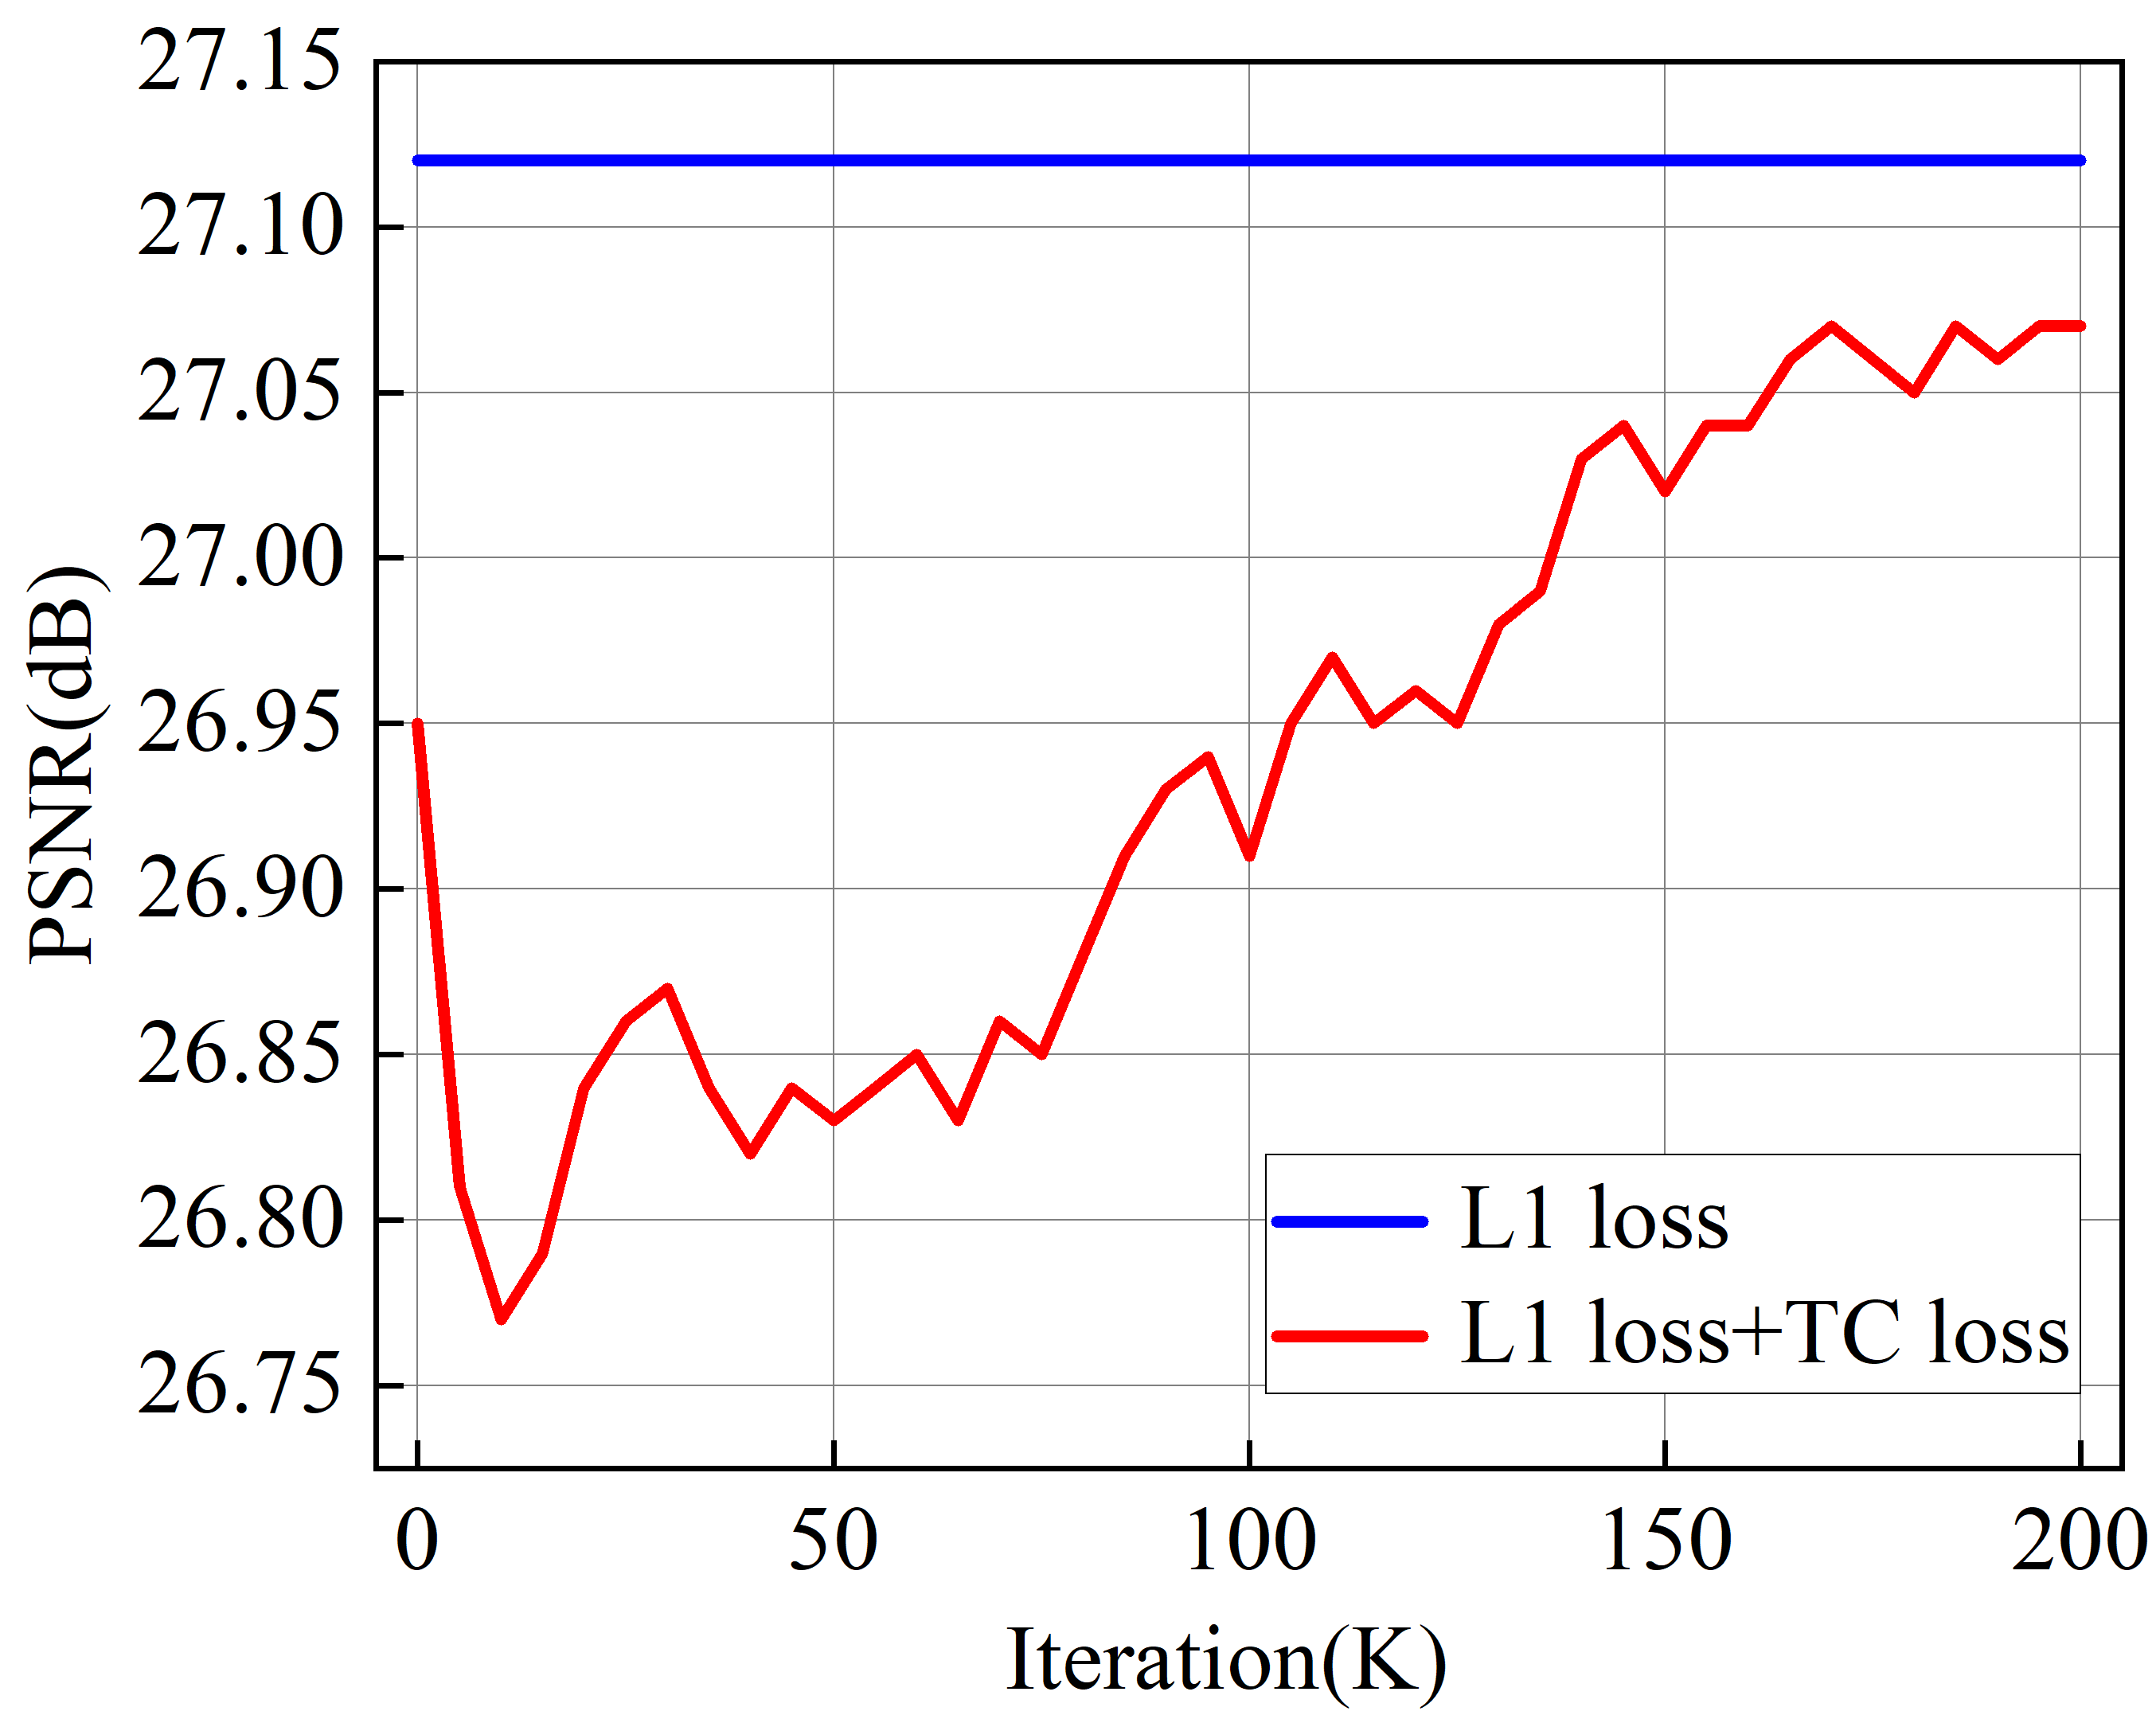
\includegraphics[width=4cm]{TCloss(PSNR).png}}
\subfigure[FLPOs with TC loss]{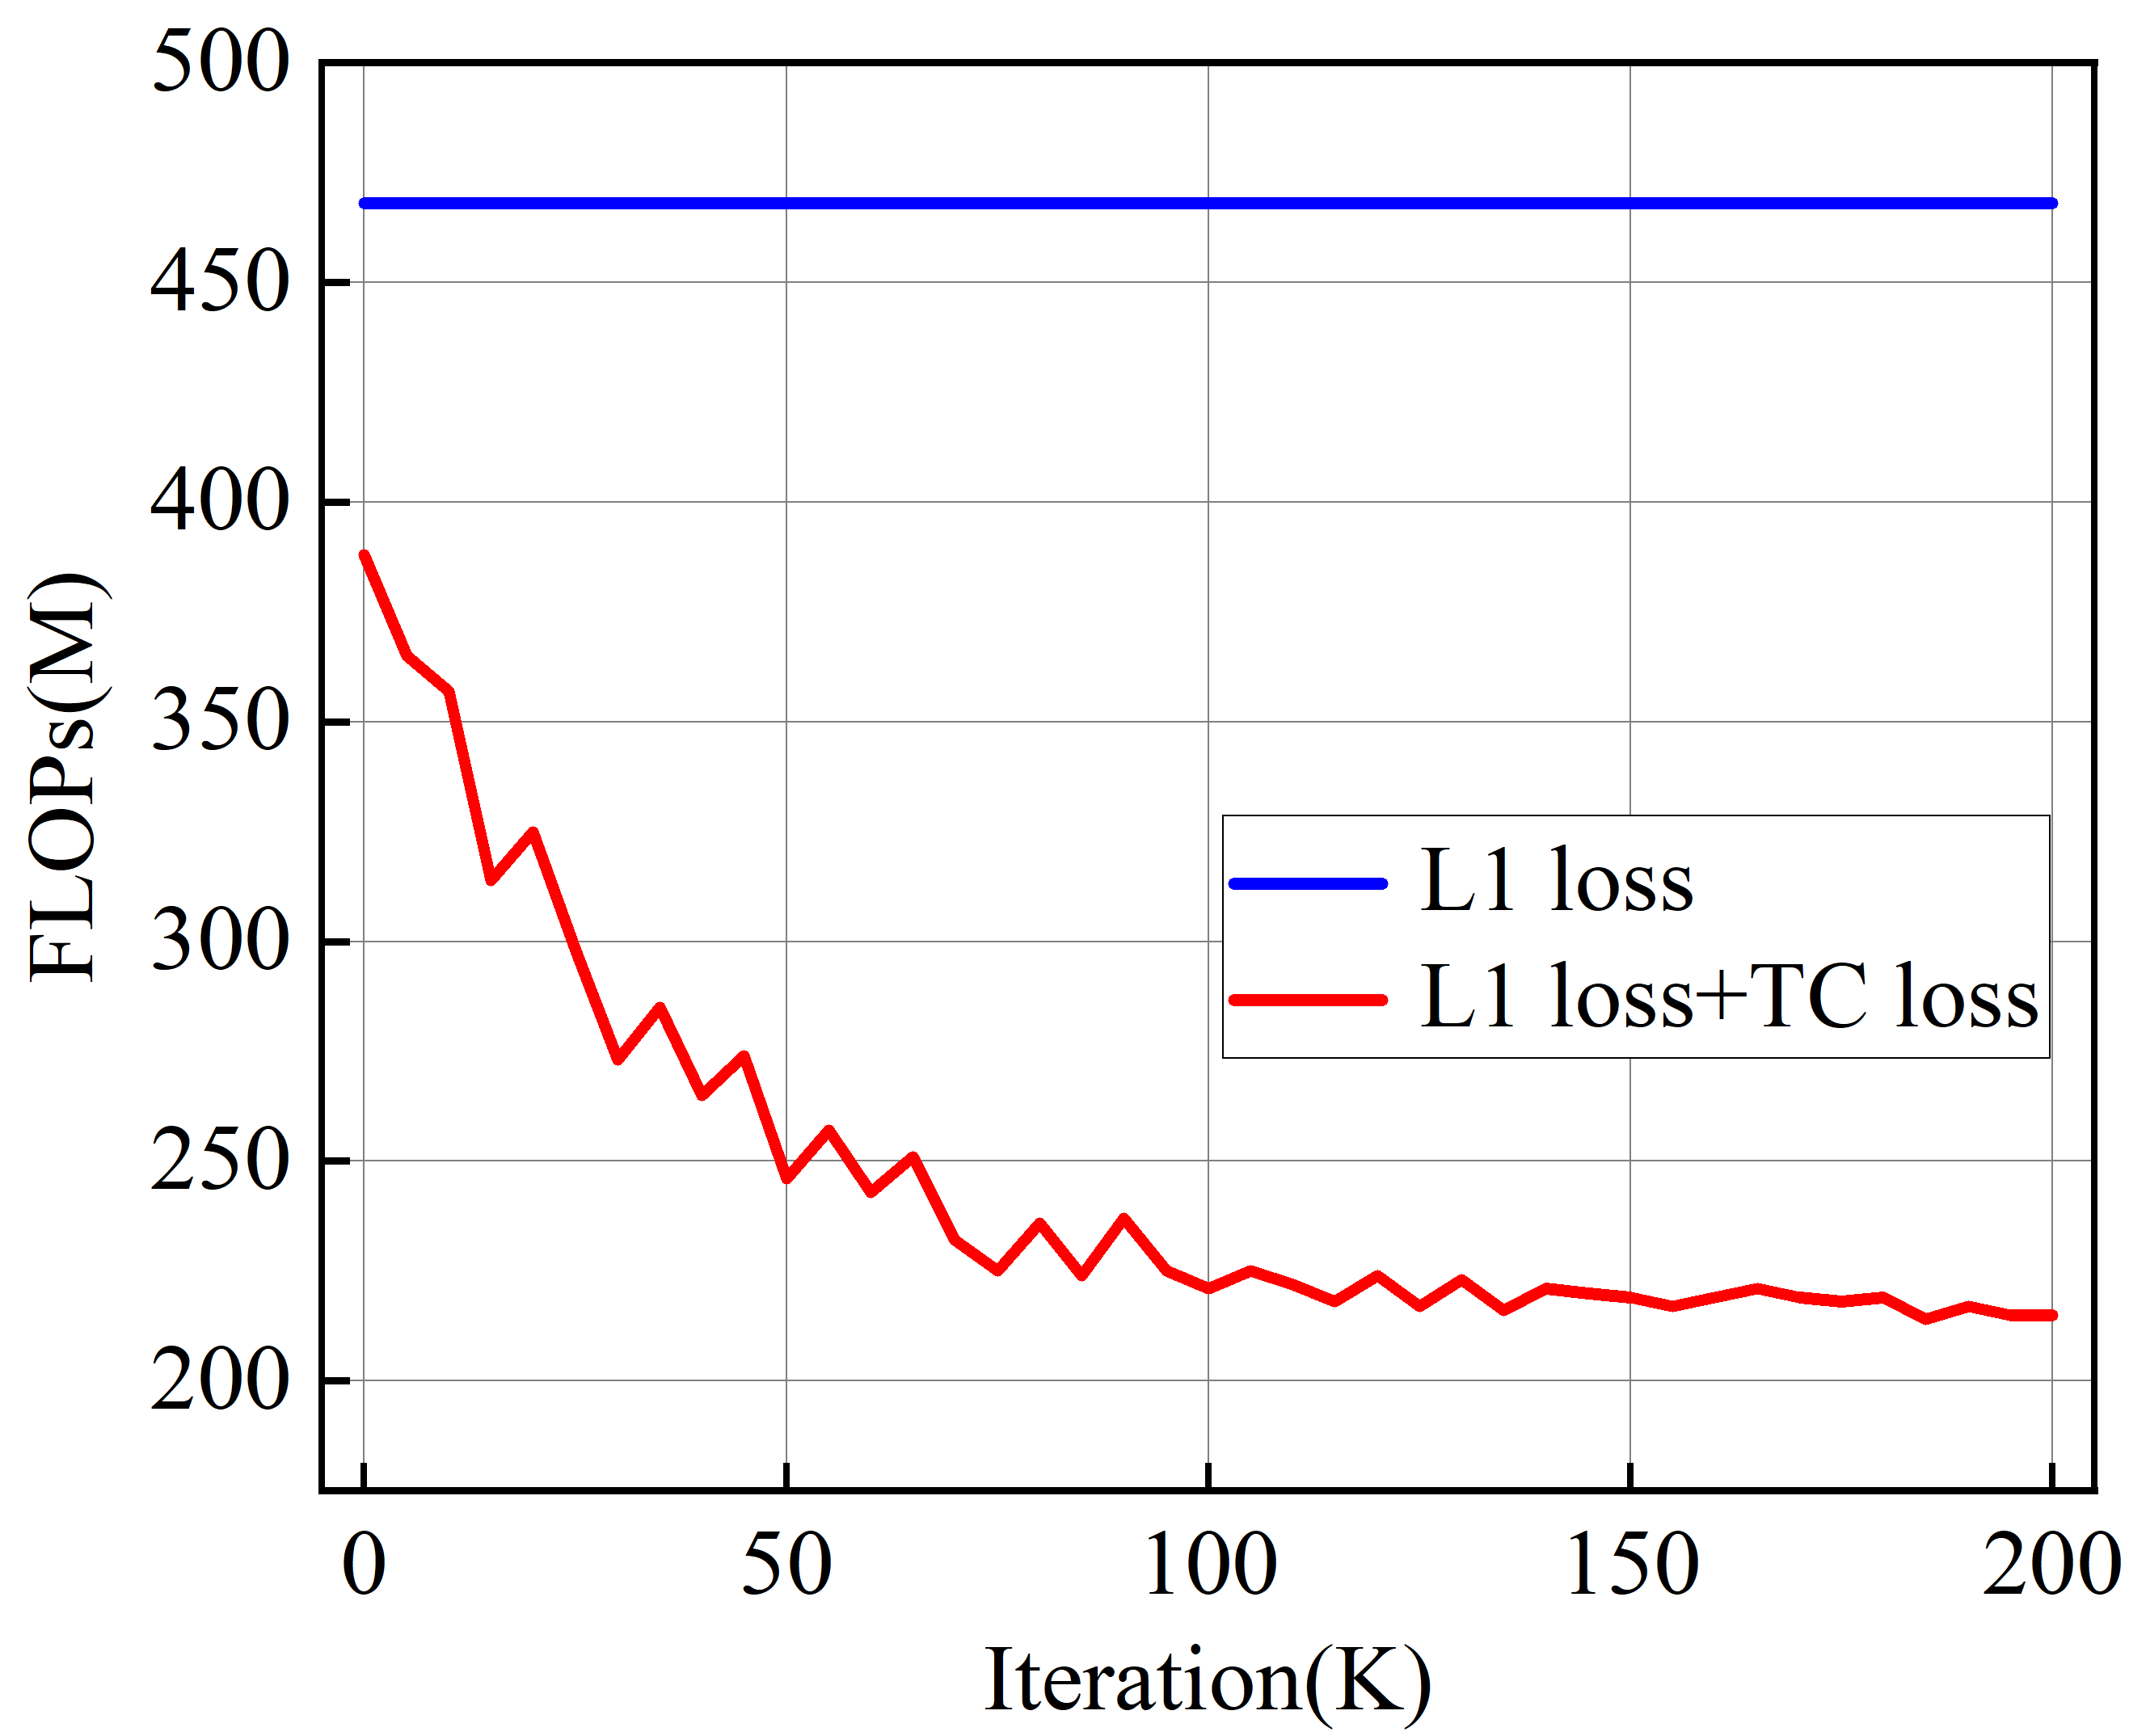
\includegraphics[width=4cm]{TCloss(FLOPs).png}}
\caption{Training curves comparisons of TA-Module with $\ell_1$ loss and $\ell_1$ loss+TC loss for FSRCNN-TARepSR.} 
\label{fig:TCloss}  
\end{figure}
% \vspace{-1.1cm}

\begin{figure*}
	\centering
	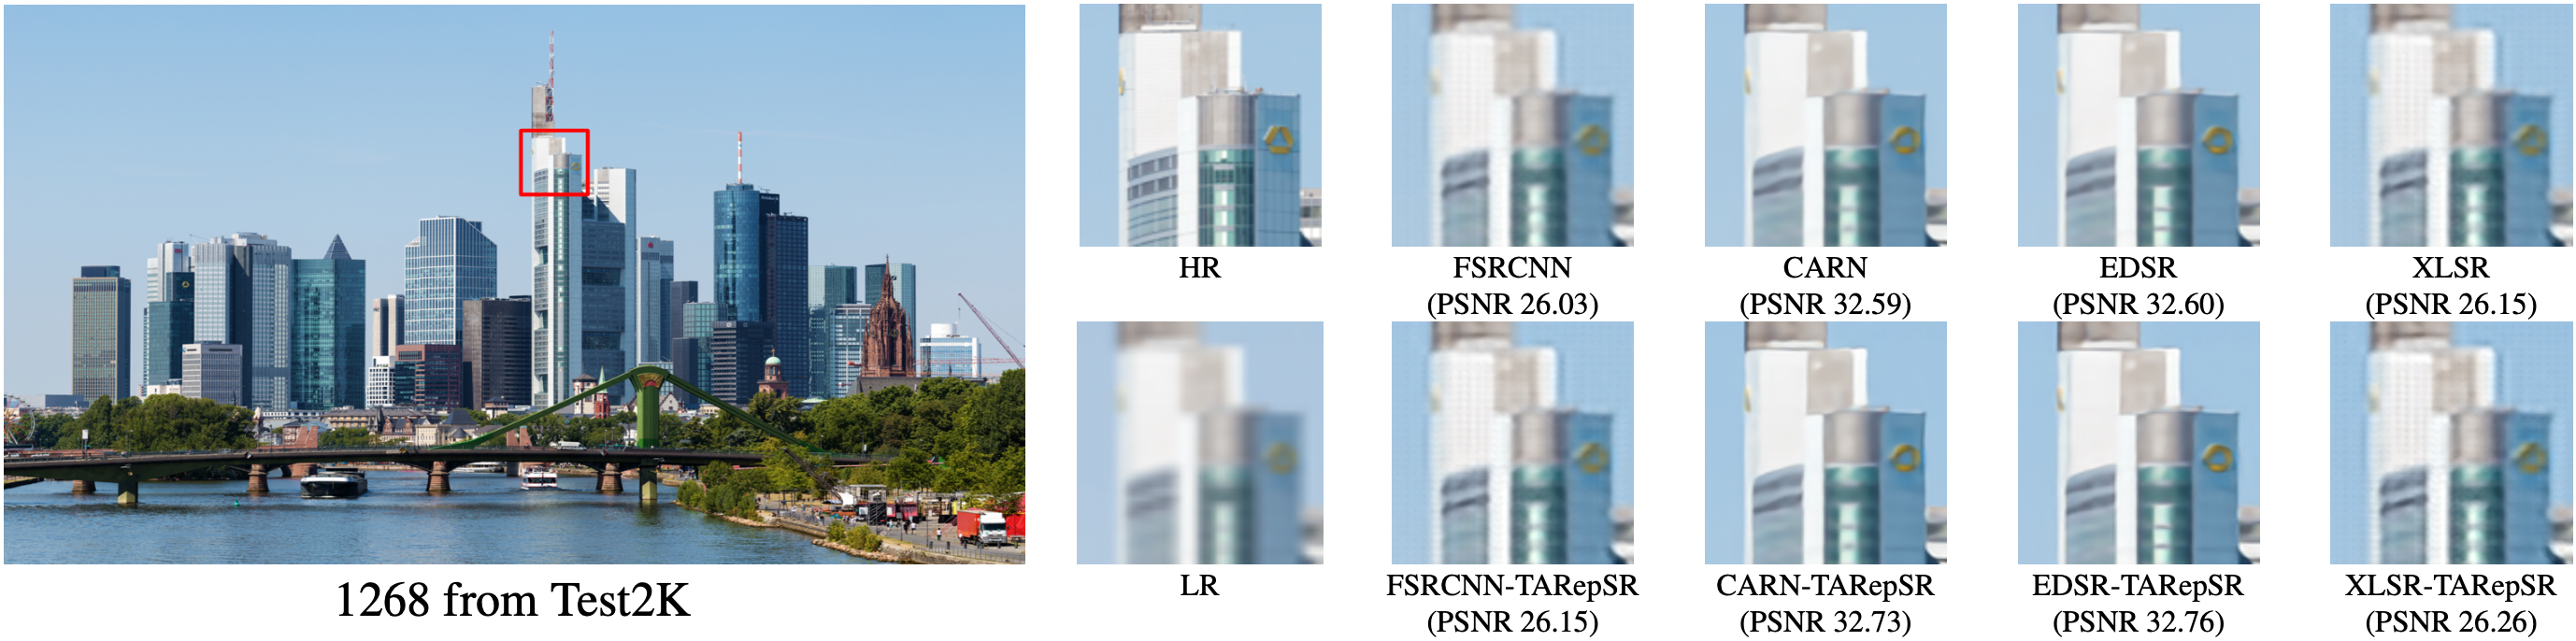
\includegraphics[width=4.6in]{1268.png}
	\\
	\centering
	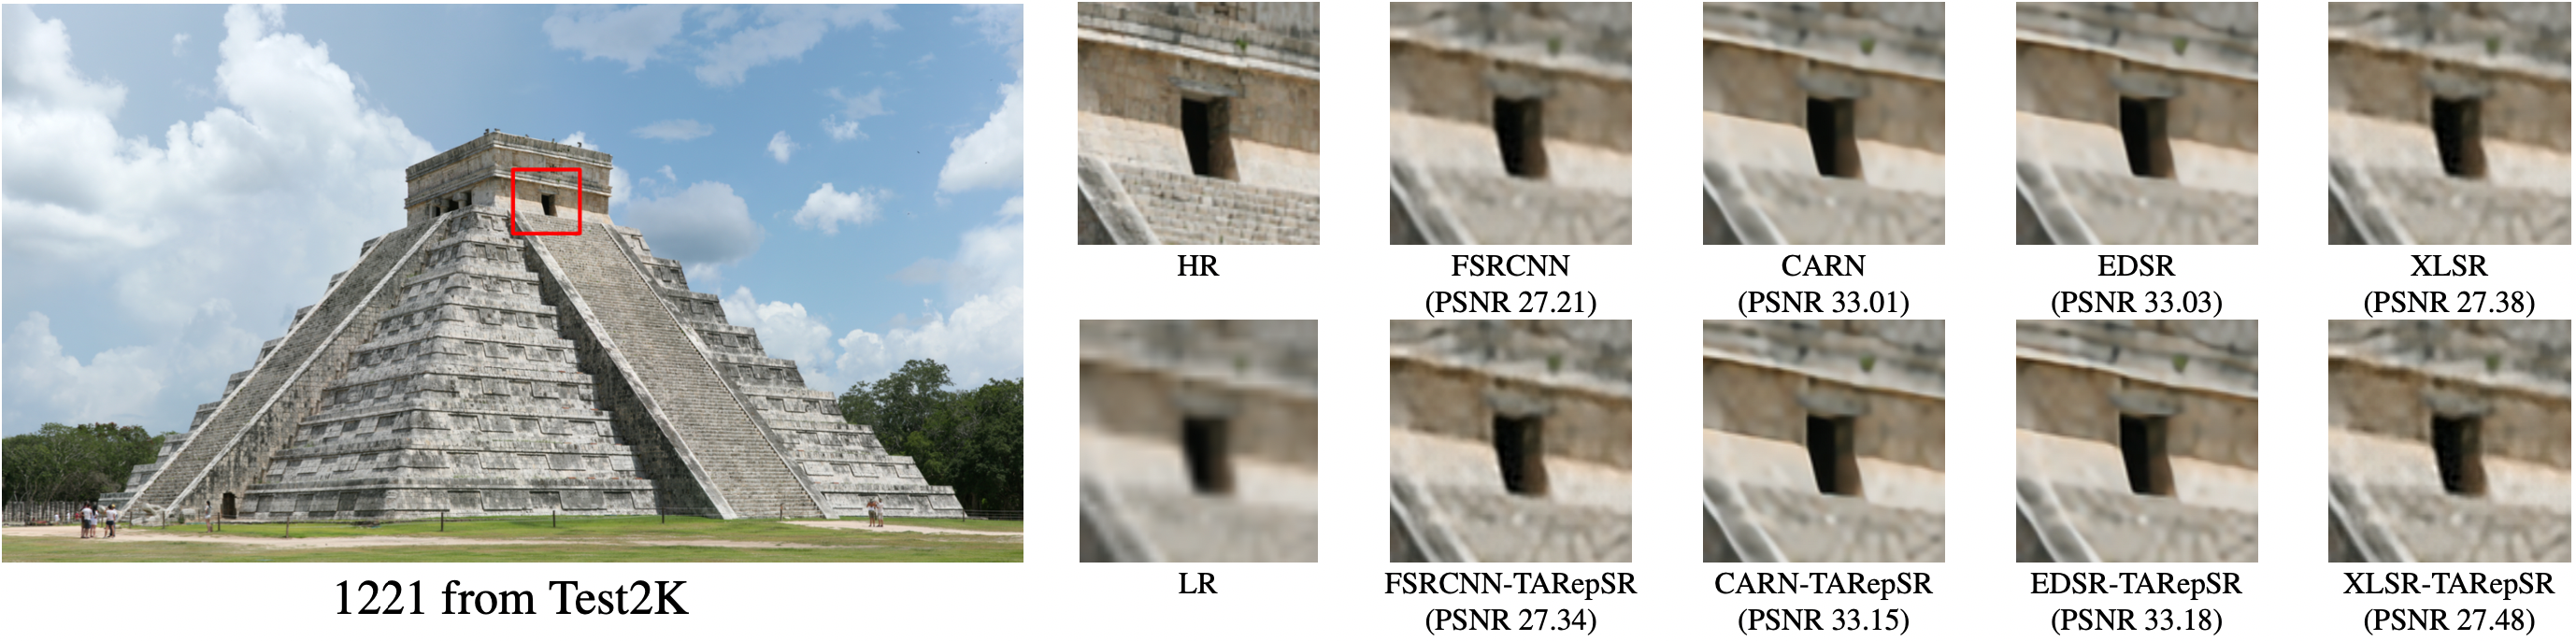
\includegraphics[width=4.6in]{1221.png}
	\\
	\centering
	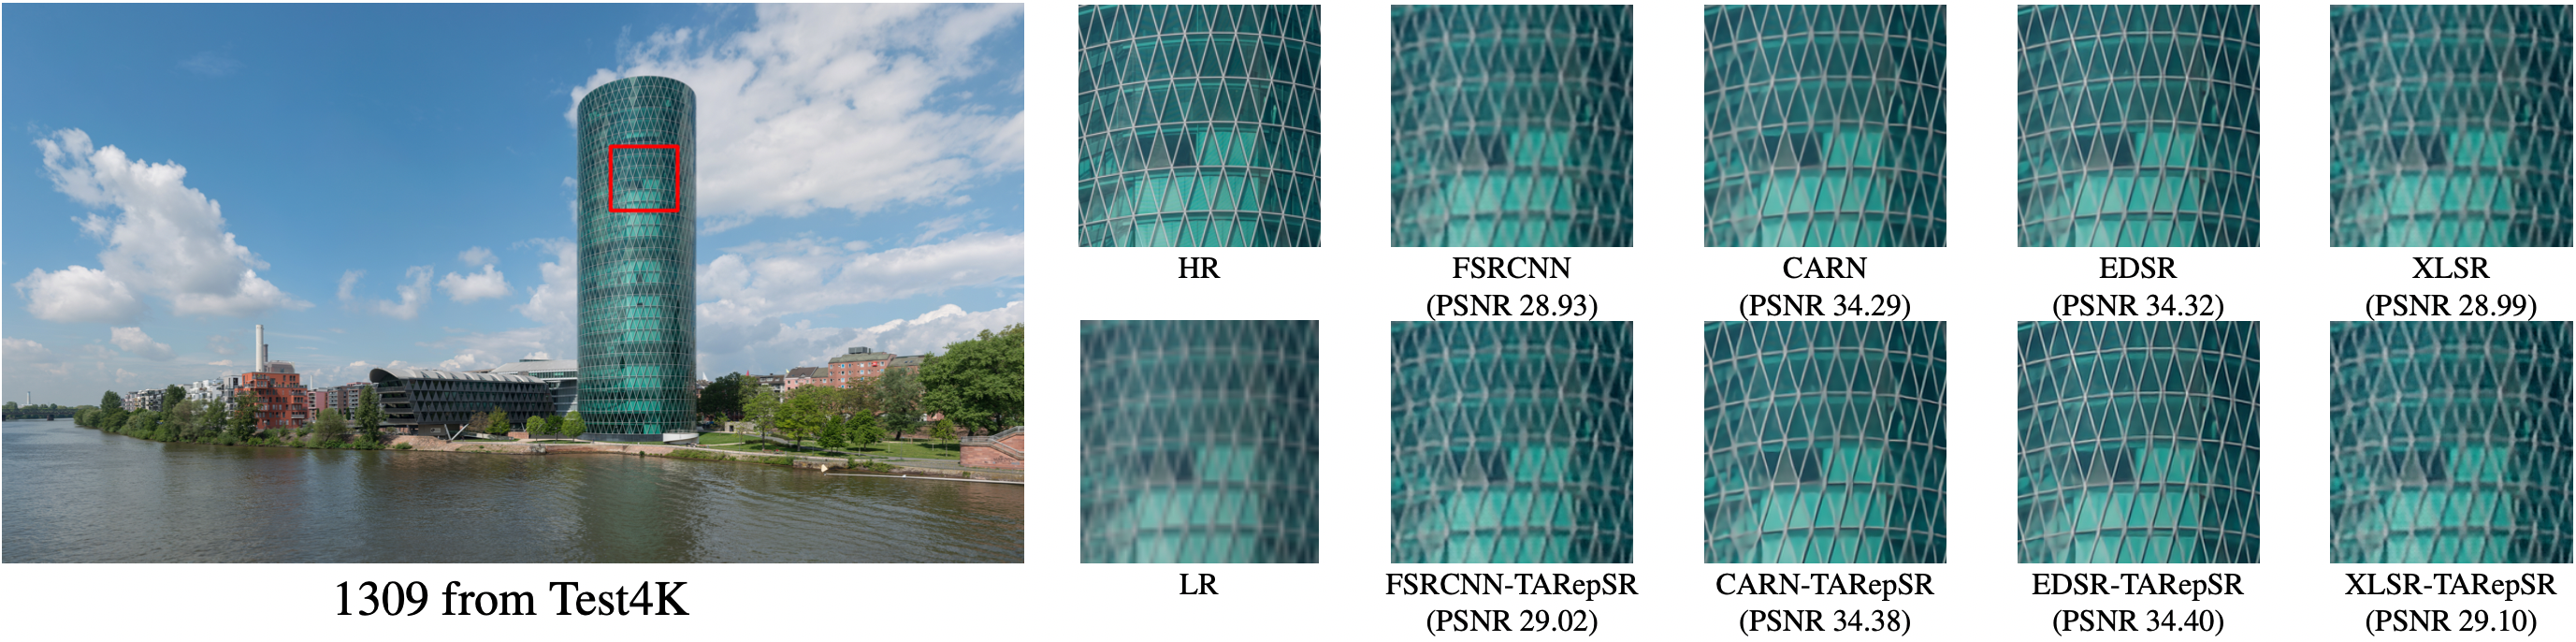
\includegraphics[width=4.6in]{1309.png}
	\\
	\centering
	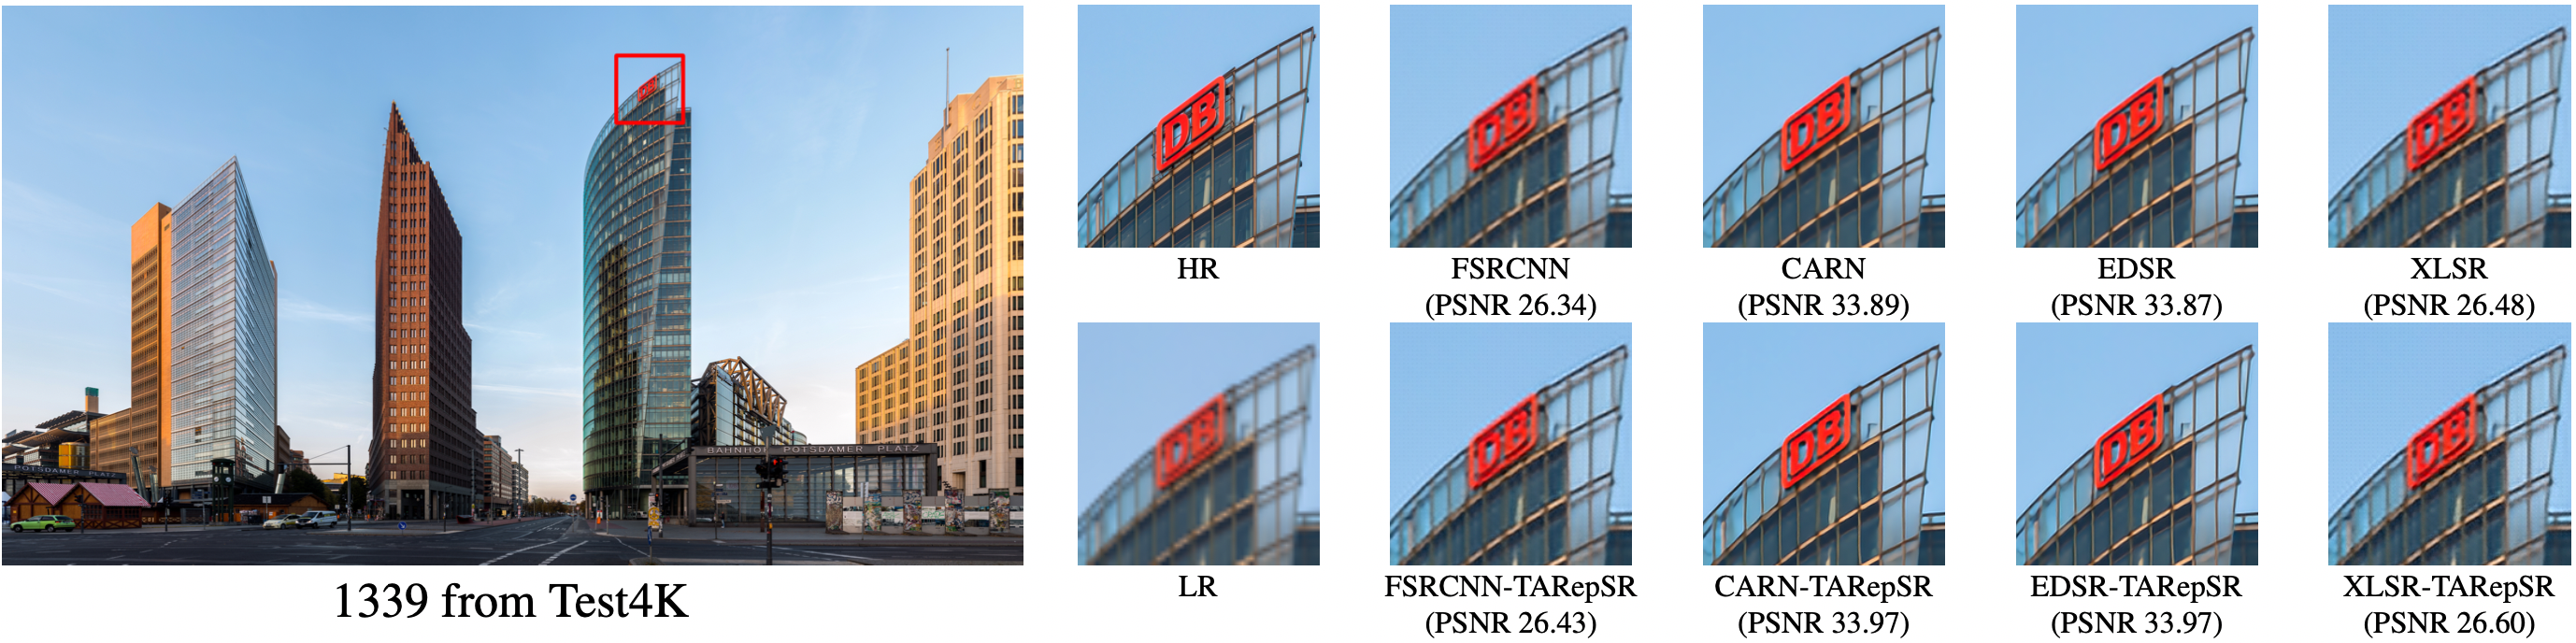
\includegraphics[width=4.6in]{1339.png}
    \\
    \centering
	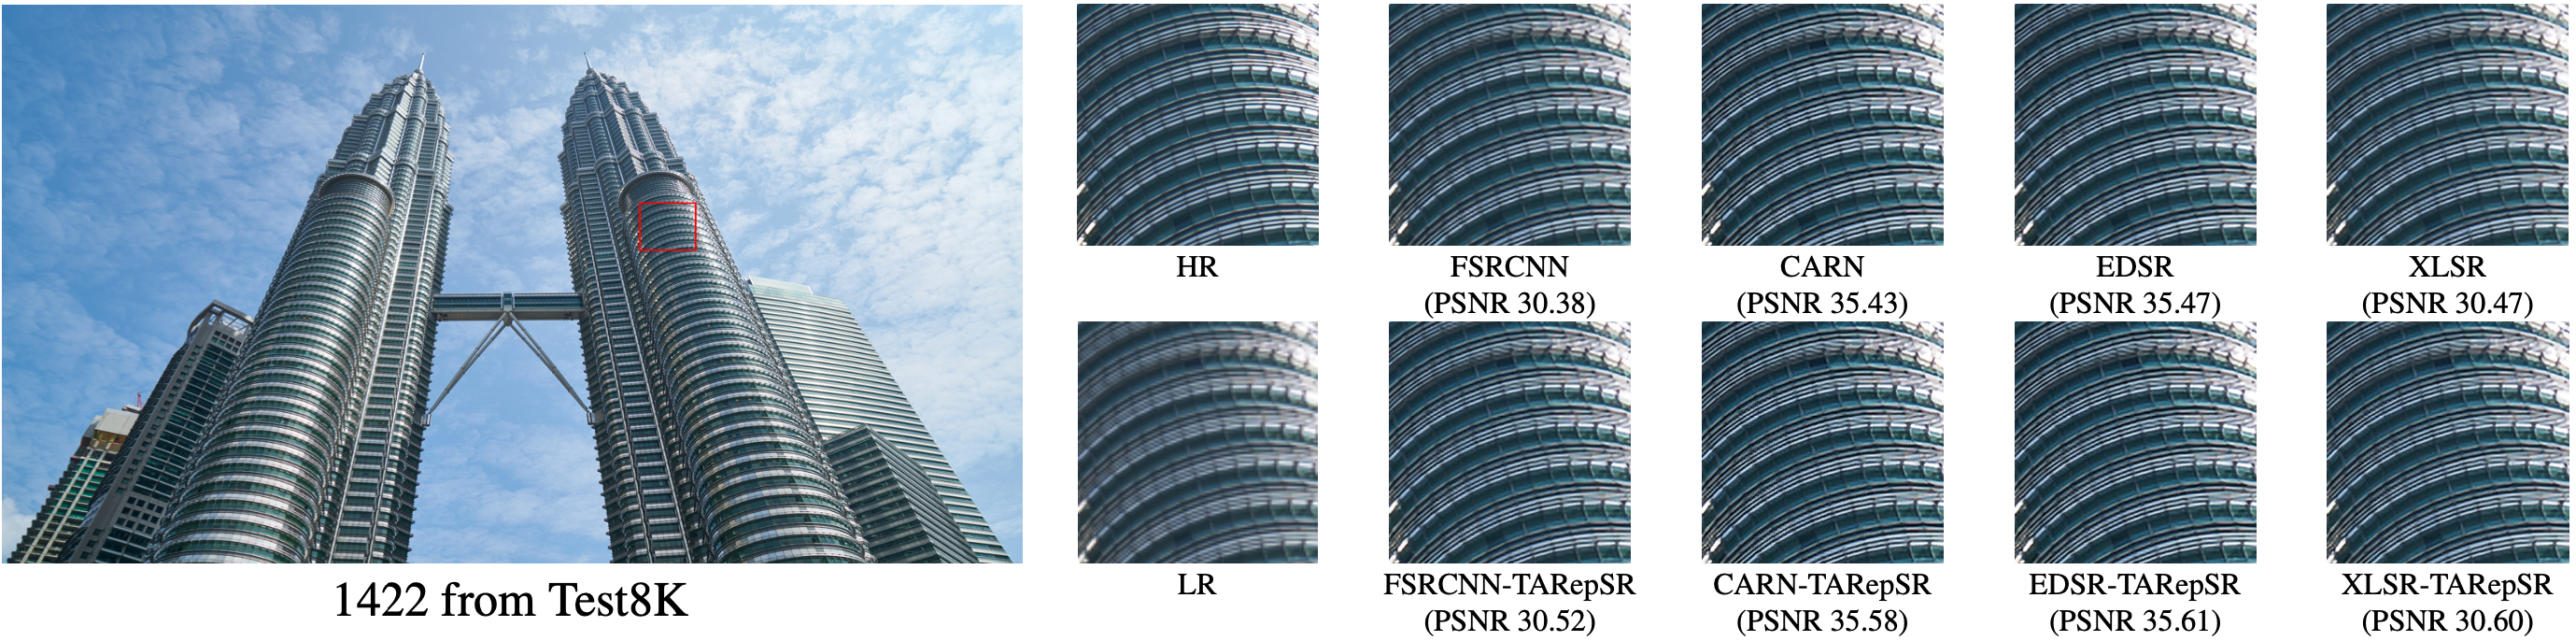
\includegraphics[width=4.6in]{1422.png}
	\\
	\centering
	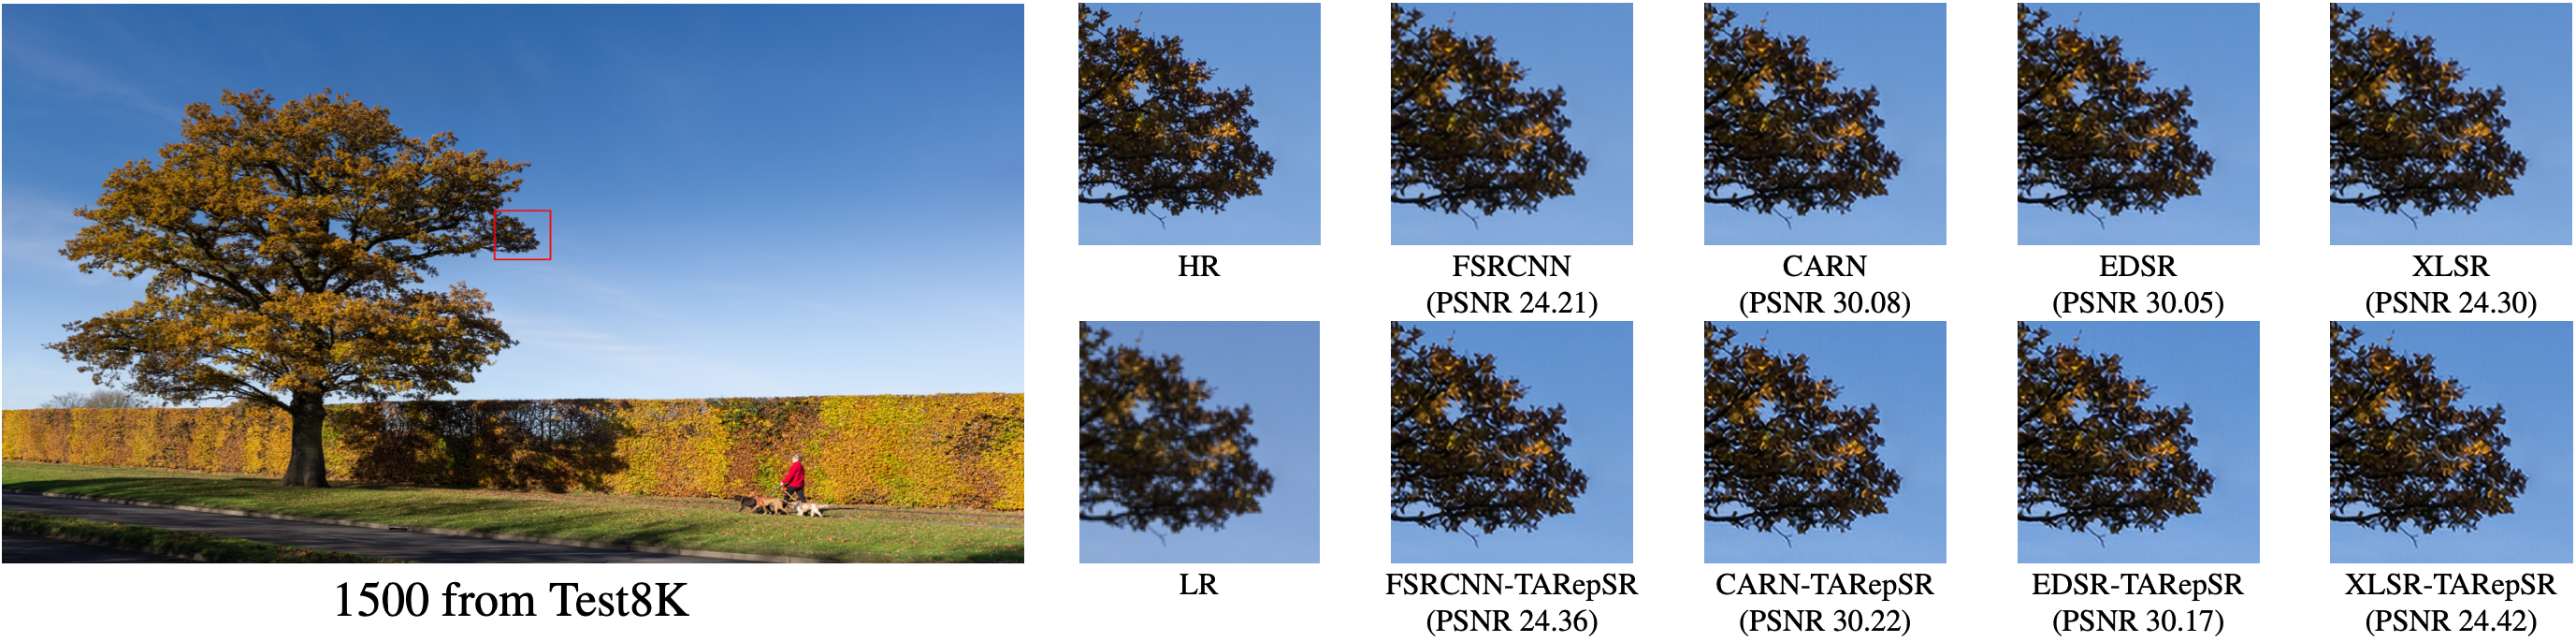
\includegraphics[width=4.6in]{1500.png}
	\caption{Visual results of TARepSR and the original networks on 8K images for upscaling factor $\times$4.}
\label{resultImage}
\end{figure*}

\subsection{Effectiveness of TC loss}
In this section, we compare the PSNR and FLOPs of $\ell_1$ loss and $\ell_1$ loss+TC loss with the number of iterations (see Figure~\ref{fig:TCloss}) to test the effectiveness of the proposed TC loss on SR performance. As seen in Figure~\ref{fig:TCloss}, the PSNRs and FLOPs of the $\ell_1$ loss converge to stability early because all sub-images are defined as complex textures. However, the PSNRs and FLOPs, after the introduction of TC loss, look normal because it makes the texture classification more inclined to ``Smooth'' and ``Medium'' to avoid getting into a bad local minimum in the optimization.

\subsection{Regarding the latency} 
TARepSR splits the complete image into several patches. The different patches can be considered a small LR image and processed in parallel. When a single GPU is used for inference, four components affect the inference time of TARepSR, including (i) sub-image decomposition, (ii) TA-Module, (iii) VarRepSR-Module, and (iv) sub-image combination. Regarding (i) and (iv), we use simple image processing methods provided by Pytorch with negligible computational cost. Regarding (iii), the difference compared to the existing SR network is that the VarRepSR-Module super-resolves several sub-images separately. Based on the characteristics of SR and reparameterization, it is known that the computational cost of SR is similar when the number of pixels in all sub-images is the same as the number of pixels in the original image.

Further, to analyze the latency of each component, we compared the latency before and after using TARepSR (see Table~\ref{Latency}). As shown in Table~\ref{Latency}, the difference between before and after using TARepSR is mainly in the computational cost of the TA-Module. The TA-Module is a reasonably lightweight classification network, and its FLOPs are only about 2\% of the total. In summary, the latency introduced by TARepSR is acceptable.

\begin{table}[h!]
\caption{Latency of TARepSR's components on Test2K}
\label{Latency}
\centering
\begin{tblr}{
  cells = {c},
  row{2} = {fg=MineShaft},
  row{3} = {fg=MineShaft},
  cell{1}{1} = {fg=MineShaft},
  cell{1}{2} = {c=2}{fg=MineShaft},
  cell{2}{1} = {r=2}{},
  cell{2}{2} = {c=2}{},
  cell{2}{4} = {r=2}{},
  cell{3}{2} = {c=2}{},
  cell{4}{1} = {r=2}{fg=MineShaft},
  cell{4}{4} = {r=2}{fg=MineShaft},
  vline{2-4} = {1-2}{},
  vline{2-4} = {3}{},
  vline{2-4} = {4}{},
  vline{2-4} = {5}{},
  hline{1-2,4,6} = {-}{},
}
Model           & Part of FLOPs &                 & Sum of FLOPs \\
FSRCNN          & super-resolution       &                 &  468M        \\
                & 468M                   &                 &              \\
FSRCNN-TARepSR  & TA-Module              & VarRepSR-Module &  480M        \\
                & 11M                    & 469M            &              
\end{tblr}
\end{table}


\subsection{Reasonableness of the image being decomposed into several patches}
\textbf{Inconsistency along patch borders.} First, a complete image is split into several patches and processed with three different weights, which means there may be inconsistencies along patch borders. However, we believe that the bias due to inconsistency is negligible. Our analysis is shown as follows.

(1) TARepSR framework divides the image into smooth, medium, and complex regions with different weights, which means there may be inconsistencies in the intersections of the different regions. As shown in Figure~\ref{boundaries}, the red line indicates where biases may exist, which account for $\sim$10\% of the boundaries of all patches.

\begin{figure}
    \centering
    % \setlength{\abovecaptionskip}{0.cm}
    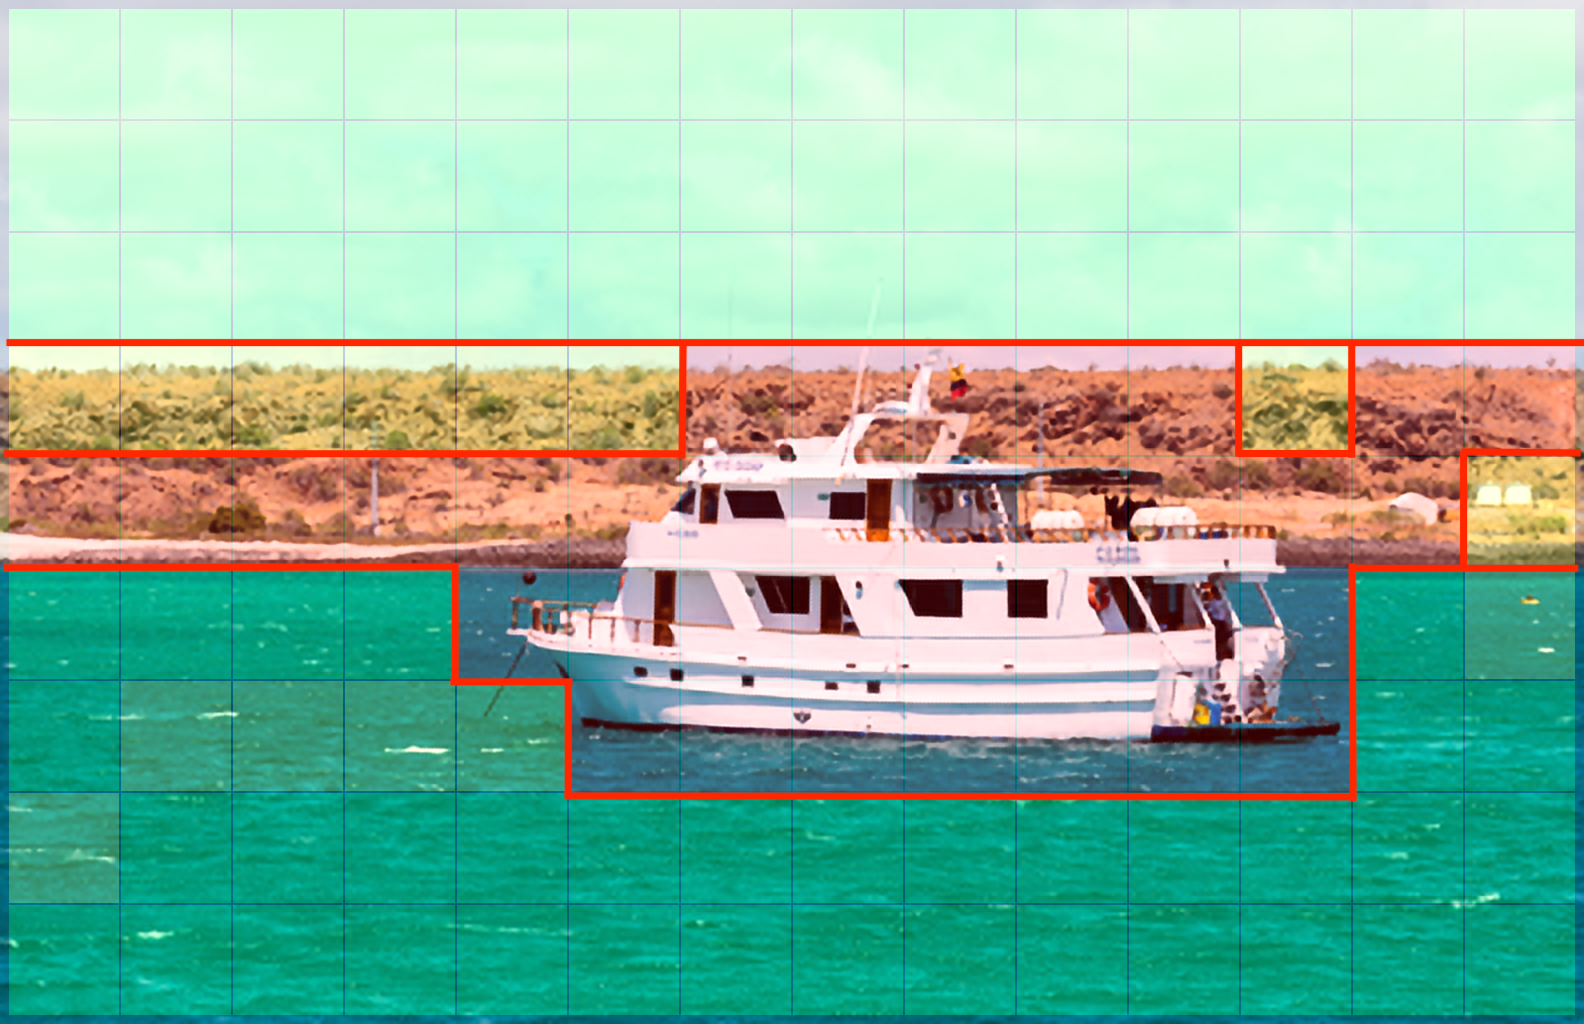
\includegraphics[width=2.5in]{1217_mask_edge.png}
    \caption{The boundaries of ``1217" (DIV8K) where biases may exist.}
    \label{boundaries}
\end{figure}

(2) Our framework is designed to process 4K/8K images, and the pixels at the boundaries where errors may exist are only $\sim$0.01\% to $\sim$0.05\% of the whole image. In Figure~\ref{junction}, the same weights are used to process Figure~\ref{junction} (a), (b), (e), and (f), VarRep-S is used in Figure~\ref{junction} (c), (g) and VarRep-L is used in Figure~\ref{junction} (d), (h). It is not easy to see the difference from the visualization results.

\begin{figure}
    \centering
    % \setlength{\abovecaptionskip}{0.cm}
    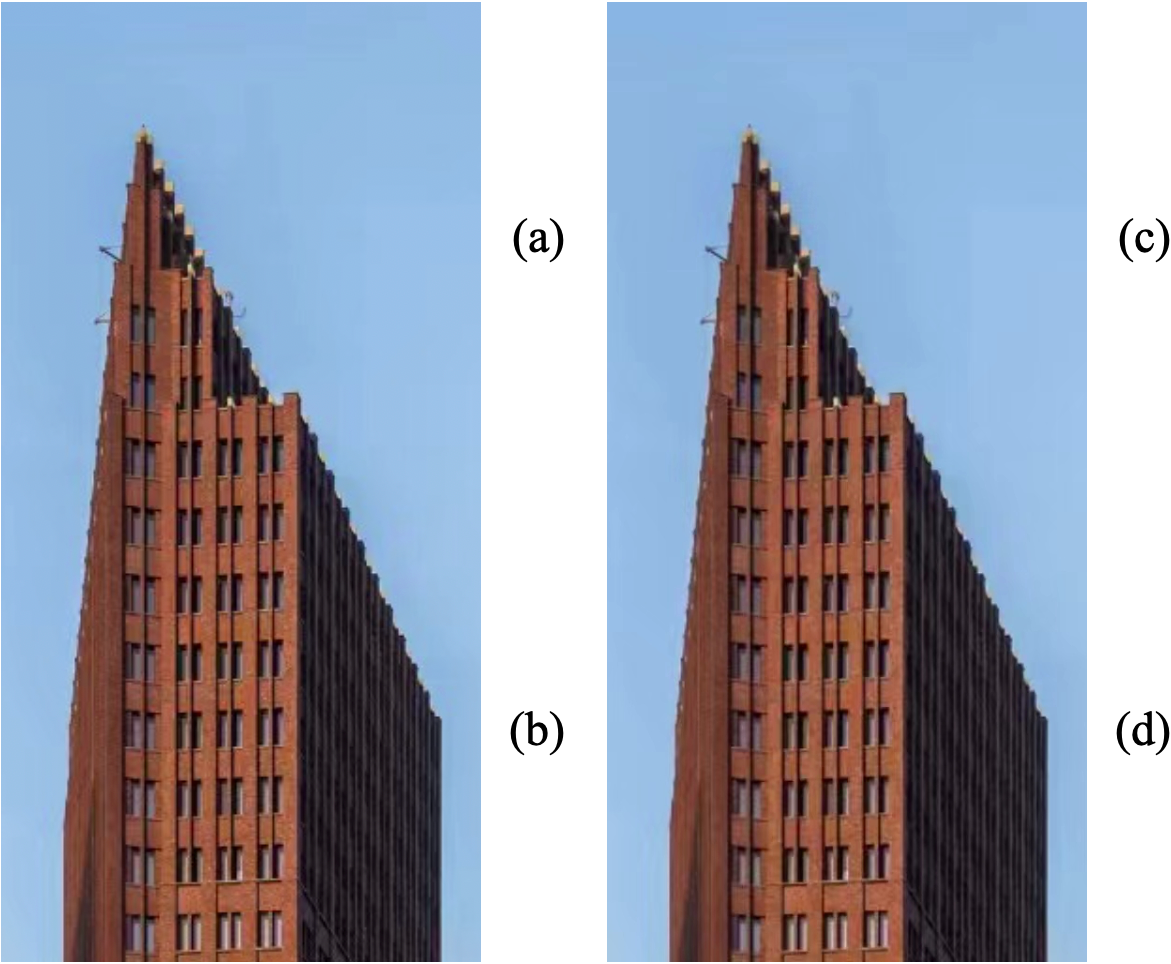
\includegraphics[width=2.3in]{1339_cons.png}
    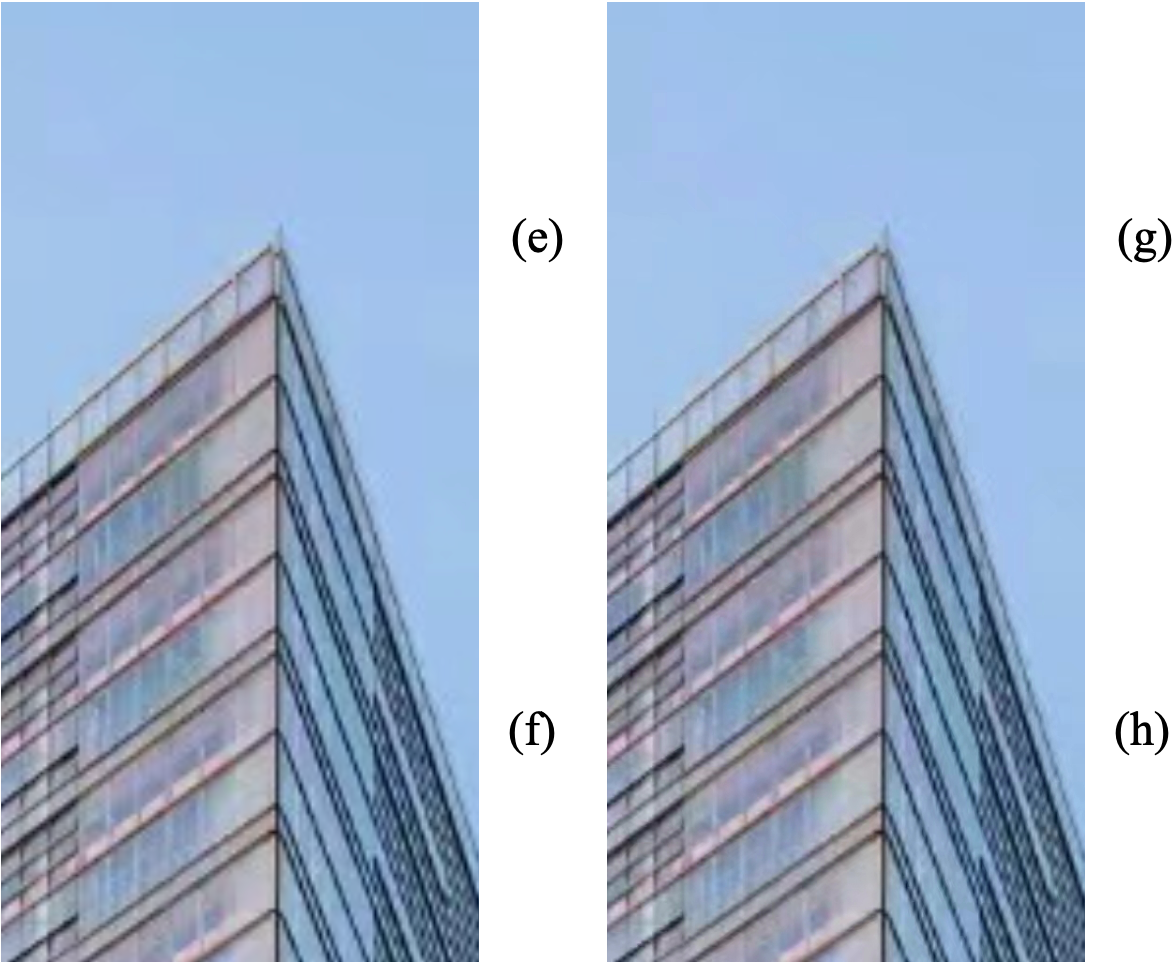
\includegraphics[width=2.3in]{1339_cons2.png}
    \caption{Comparison of the junction of regions with different textures.}
    \label{junction}
\end{figure}

In summary, the above error is negligible, but it is indeed a detail that can be optimized and may be solved in the future.


\subsection{Other Applications}
First, TARepSR is applied to the actual image of the classroom to verify the effectiveness of TARepSR on real images. As shown in Figure~\ref{real-images}, the image's texture using TARepSR is sharper than the original image. In addition, the SR method can be seen as a plug-and-play module, which can be used in the first step of advanced computer vision, such as target detection and semantic segmentation, to improve their performance.

\begin{figure}
    \centering
    % \setlength{\abovecaptionskip}{0.cm}
    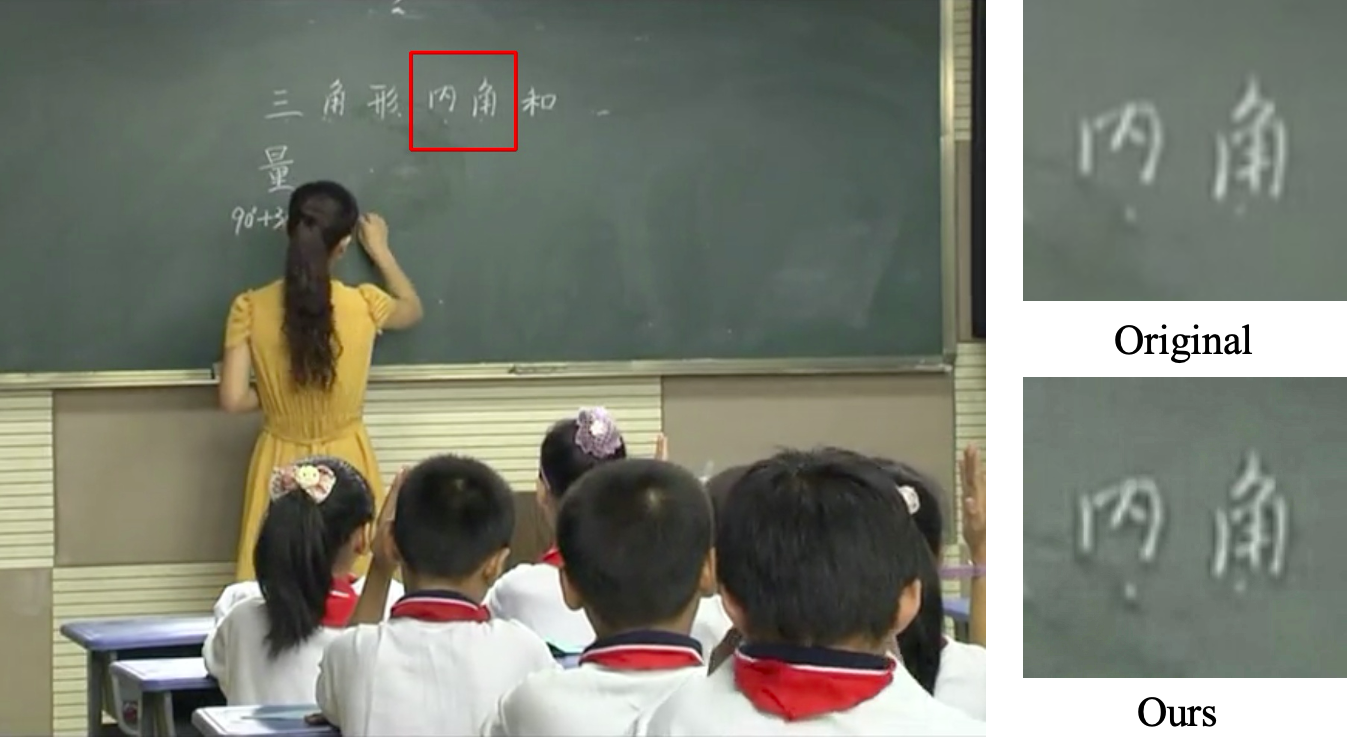
\includegraphics[width=2.3in]{65147_contrast.png}
    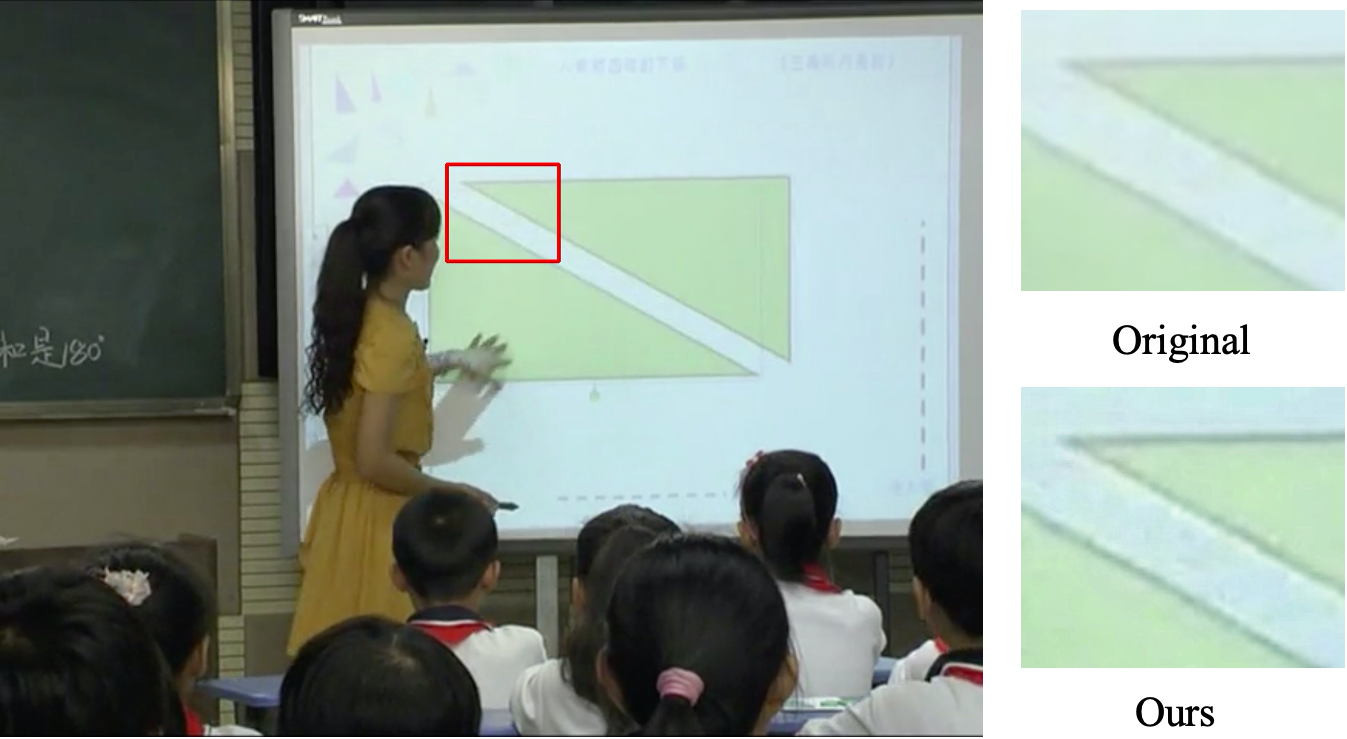
\includegraphics[width=2.3in]{65305_contrast.png}
    \caption{Comparison on real images of classroom}
    \label{real-images}
\end{figure}

\section{Conclusion}
In this paper, we explored the effectiveness of Rep techniques in regions with different textures and proposed a texture-aware ``Local-Rep'' strategy rather than ``Global-Rep''. Then, we proposed a general TARepSR framework using the ``Local-Rep'' strategy, which aims to improve the imaging quality of SR on 4K/8K images with negligible increase in computational cost and alleviate the accuracy drop after quantization. Finally, we proposed a TC loss to classify different textures better. Experimental results show that the TARepSR framework can improve the imaging quality of existing SR networks by $\sim$0.1dB on 4K/8K images with negligible increase in computational cost. In addition, the accuracy drop of our strategy after quantization is reduced by $\sim$0.15 on average compared to the SOTA SR methods based on ``Global-Rep''.

\section*{Declarations}
\textbf{Conflict of interest statement:} The authors declare no conflicts of interest.
\textbf{Data availability statement:} The data supporting this study's findings are available from the corresponding author upon reasonable request.

\bibliography{sn-bibliography}

\end{document}
